\documentclass[11pt,a4paper,notitlepage]{article}
\usepackage[utf8]{inputenc}
\usepackage{amsmath}
\usepackage{amsfonts}
\usepackage{csvsimple}
\usepackage{amssymb}
\usepackage{hyperref}
\hypersetup{
    colorlinks=true,
    linkcolor=black,
    filecolor=black,
    urlcolor=cyan,
    citecolor=black,
}
\usepackage{tikz}
\usetikzlibrary{calc,patterns,angles,quotes,shapes.geometric, arrows}

\def\layersep{2.5cm}
\def\layersepSmall{1.2cm}

\tikzstyle{train} = [rectangle, rounded corners, minimum width=2.2cm, minimum height=1cm,text centered, draw=black, fill=red!30]
\tikzstyle{test} = [rectangle, rounded corners, minimum width=2.2cm, minimum height=1cm,text centered, draw=black, fill=green!30]
\tikzstyle{data} = [rectangle, rounded corners, minimum width=11.8cm, minimum height=1cm,text centered, draw=black, fill=gray!30]
\tikzstyle{MSE} = [rectangle, rounded corners, minimum width=1.4cm, minimum height=1cm,text centered, draw=black, fill=orange!30]
\tikzstyle{arrow} = [thick,->,>=stealth]

\usepackage{float}
%\usepackage{mathtools}
\usepackage{bm}
\usepackage[margin=1in]{geometry}

\title{Project 3 in FYS-STK415\\ \large Using Machine Learning to calculate atomization energies}
\author{Simon Elias Schrader }
\date{Autumn 2020}
\usepackage{hyperref}

\usepackage{natbib}
\usepackage{graphicx}
\graphicspath{{../figures/presentable_data/}} %Setting the graphicspath

\begin{document}

\maketitle
\tableofcontents
\listoffigures
\listoftables
\clearpage
\begin{abstract}
Predicting molecular properties as function of the molecular structure is an important part of Computational and Theoretical Chemistry. Using ab-initio methods, however, is computationally very expensive.As lots of molecular properties such as atomization energy of chemicals are easily available for a vast number of molecules, we used different Machine Learning techniques to predict the atomization energies of a set of molecules which are represented with their Coulomb matrix. We found that Tree-based approaches work well, and got a 5-fold Cross-validated test Mean Absolute Error (MAE) of 13.05 kcal/mol using a Single Decision Tree. With Tree Bagging/Random Forests, we managed to reduce that error to 10.20 kcal/mol, while Tree Boosting gave an error of 6.07 kcal/mol. We did not manage to find good parameters for the Neural Network and got a test MAE in the same range as for a Single Decision tree, though we know it is possible to find those \citep{Atomization_network}, and we found that Ridge regression yields unsatisfactory results ($MAE \approx 20$ kcal/mol). We analyzed how well molecules can be represented when Hydrogen atoms are removed and found that the test MAE with Boosting is around 27.5 kcal/mol. We performed a Principal Component Analysis on the data and found that while there are linear dependencies, however the variance is not strongly dominated by few Principal Components. 
\end{abstract}
\section{Introduction}
In this article, we analyse how different machine learning techniques can be used to predict the atomization energy of organic molecules. We implemented Ridge Regression, Feed Forward Neural Networks, Decision Trees, Random Forests, Decision Tree Bagging \&  Boosting. Boosting and Neural Networks are known for their accuracy \citep{hastie}, while Linear Regression (including Ridge Regression) and Decision Trees are easy to interpret. Bagging and Random Forests can be considered a natural step between Decision Trees and Boosting. For Neural Networks and the Tree-based learning methods, we compare different parameters, such as the learning rate (for boosting and Neural Networks), Tree depth and Number of Trees. \\There are many ways to represent a molecule on a computer, and we used Neural Networks to compare these different approaches - either by the position and charge of atoms, or by their Coulomb matrix, which can be further reduced. For the other algorithms, we only used the approach which gave the best results in Neural Networks - the reduced Coulomb matrix. We also tested how important it is to include Hydrogen atoms in the molecular representations, as these have specific attributes that make them less important than other atoms. They are also the most prevalent atom, and removing them gives a large speedup for the learning algorithms. We performed a Principal Component Analysis to explore whether the feature space might be dominated by few orthogonal features. This was done both for whole molecules as well as for the ones with Hydrogen removed. Finally, we compared the Ridge Regression analysis and the Neural Network analysis to earlier research on the same data set \citep{Atomization_network,Atomization_Ridge}.\\
In the Methods \& Theory part, we first describe the data set, what it is and what the parameters and targets mean, and where it is obtained from. We then describe the different ways to represent molecules and justify why machine learning can be used to predict atomization energies. We then go on and explain the different Regression algorithms and important statistical concepts used in this article . After that, we explain to approaches to reduce features space - Principal Component Analysis \& why it can be argued for that Hydrogen atoms can be removed without losing too much predictability. We then explain how the algorithms were implemented computationally. In the Results part, we present the results of the different algorithms and assess them critically. We also compare our results to results obtained in earlier research. Finally, we share our conclusions about the results we have found. \\\\All methods are implemented using the Python programming language. The programs are available at the \href{https://github.com/schraderSimon/FYS-STK/tree/master/project3}{Github address}. 
\section{Methods \& Theory}
\subsection{Data set}
The data set \citep{blum,Atomization_Ridge}, which can be downloaded from \href{http://quantum-machine.org/datasets/}{quantum-machine.org}, consists of the nuclear charges  and and the atomic positions (in atomic units) of 7165 molecules consisting of up to 23 molecules which serve as predictors (or a place to start for new predictors). The target value is the atomization energy, which is defined as the energy which is necessary to atomize the molecule, that is, it is the energy difference between the molecule's ground state energy and the ground state energy of the atoms composing it, it can hence be thought of as the potential energy that is "stored in the chemical bonds" and ranges from -800 to -2000 kcal/mol. Due to the size of the molecules, exact ground states and exact ground state energies that are the solution to the electronic Schrødinger equation, are not easily available, instead, atomization energies were approximated using Density Functional Theory with the PBE0 functional. \\
The data is pre-split into 5 randomly sorted subsets of equal size, which allows for an easy implementation of Cross-Validation. An explanation of Cross Validation can be found in \citep{Project2}.
\subsubsection{The Coulomb Matrix}
In reality, molecular energies are invariant under translations and rotations of atomic positions. For this reason, atomic positions are not a suitable predictor for Machine Learning, and the data set needs to be transformed into a predictor that is translation \& rotation invariant. We define the Coulomb matrix C:
\begin{equation}\label{Coulomb_matrix}
\begin{split}
    & C_{ii}=0.5Z_i^{2.4}\\
    & C_{ij}=\frac{Z_iZ_j}{|r_i-r_j|}\;\;\; for\; i\neq j
\end{split}
\end{equation}
Where $Z_i$ is the nuclear charge and $r_i$ the atomic position. Observe that this increases the number of predictors from $4N$ to $N^2$ where N is the maximum number of atoms. This matrix is clearly invariant under translations and rotations. However, it has to weaknesses as a predictor: It is not invariant under exchange of particle indices (several Coulomb matrices can be used to describe the same molecule). Also, due to its symmetric nature, non-diagonal predictors show up twice. Following the approach described in \citep{Atomization_network}, these problems can, to a degree, be avoided by sorting the columns of Coulomb matrix by their $L^2$ norm in descending order and only taking the lower triangular part of the matrix before unravelling the lower triangular matrix into a 1-dimensional vector of length $\frac{N(N+1)}{2}$. This will be called reduced Coulomb matrix in this text. This ensures that the resulting predictors are uniquely determined for each atom \citep{Atomization_Ridge}. A part of this article will be to compare the predicative quality of the atomic charges \& positions only with both the Coulomb matrix as given in (\ref{Coulomb_matrix}) as well as the reduced Coulomb matrix.
\subsubsection{Physical motivation}
One might wonder why the atomic positions should be able to uniquely determine the atomization energies of molecules. This is motivated quantum mechanically. Within the Born-Oppenheimer approximation \citep{szabo}, the electronic Hamiltonian is uniquely determined by the nuclear charges, the atomic positions and the number of electrons. For neutral molecules, the number of electrons is determined by the sum of the nuclear charges. With the Hamiltonian determined, the ground state wave function and the ground state eigenvalue can be determined. As this is true for atoms too (only the nuclear charge matters here), the atomization energy can be considered a function of the atomic positions and nuclear charges, justifying a Machine Learning approach.
\subsection{Mean Absolute Error \& L1 regularization}
The Mean Absolute Error (MAE) between the true target $\bm{y}$ and the estimated target $\bm{\tilde y}$  is defined as 
\begin{equation}\label{MSE}
MAE(\bm{y},\bm{\tilde y})=\frac{1}{n}\sum_i^N\left|y_i - \tilde y_i \right|=\mathbb{E}\left[|\bm{y}-\bm{\tilde y}|  \right]
\end{equation}
and can be interpreted as the average of the absolute deviation between the true target and the estimated target. Unlike the MSE \citep{Project1}, large deviations do not lead to such a strong increase in the value of the MAE. As related articles use the MAE to evaluate the goodness of their fit, we will do so, too. Using MAE as cost function can be risky as the derivative is constant, however, using dynamic learning rates or Stochastic Gradient algorithms with adaptive Learning rates should be able to circumvent this problem. \\

L1 regularization adds to the cost function a value of $\lambda||W||$, where $||W||$ is sum of the absolute values of the weight parameters in a weight matrix (for Neural Networks), and $\lambda$ is the regularization parameter (in the case of Linear Regression, we end up with LASSO \citep{Project1}). Just like with L2 loss, the aim is to avoid overfitting by penalizing large weights.
\subsection{The Covariance Matrix}
For a design Matrix $\boldsymbol{X}\in {\mathbb{R}}^{n\times p}$, 
\begin{equation}
\boldsymbol{X}=\begin{bmatrix}
x_{0,0} & x_{0,1} & x_{0,2}& \dots & \dots x_{0,p-1}\\
x_{1,0} & x_{1,1} & x_{1,2}& \dots & \dots x_{1,p-1}\\
x_{2,0} & x_{2,1} & x_{2,2}& \dots & \dots x_{2,p-1}\\
\dots & \dots & \dots & \dots \dots & \dots \\
x_{n-2,0} & x_{n-2,1} & x_{n-2,2}& \dots & \dots x_{n-2,p-1}\\
x_{n-1,0} & x_{n-1,1} & x_{n-1,2}& \dots & \dots x_{n-1,p-1}\\
\end{bmatrix}=\begin{bmatrix} \boldsymbol{x}_0 & \boldsymbol{x}_1 & \boldsymbol{x}_2 & \dots & \dots & \boldsymbol{x}_{p-1}\end{bmatrix}
\end{equation}
we can define the the covariance matrix
\begin{equation}
\boldsymbol{C}[\boldsymbol{x}] = \begin{bmatrix}
\mathrm{var}[\boldsymbol{x}_0] & \mathrm{cov}[\boldsymbol{x}_0,\boldsymbol{x}_1]  & \mathrm{cov}[\boldsymbol{x}_0,\boldsymbol{x}_2] & \dots & \dots & \mathrm{cov}[\boldsymbol{x}_0,\boldsymbol{x}_{p-1}]\\
\mathrm{cov}[\boldsymbol{x}_1,\boldsymbol{x}_0] & \mathrm{var}[\boldsymbol{x}_1]  & \mathrm{cov}[\boldsymbol{x}_1,\boldsymbol{x}_2] & \dots & \dots & \mathrm{cov}[\boldsymbol{x}_1,\boldsymbol{x}_{p-1}]\\
\mathrm{cov}[\boldsymbol{x}_2,\boldsymbol{x}_0]   & \mathrm{cov}[\boldsymbol{x}_2,\boldsymbol{x}_1] & \mathrm{var}[\boldsymbol{x}_2] & \dots & \dots & \mathrm{cov}[\boldsymbol{x}_2,\boldsymbol{x}_{p-1}]\\
\dots & \dots & \dots & \dots & \dots & \dots \\
\dots & \dots & \dots & \dots & \dots & \dots \\
\mathrm{cov}[\boldsymbol{x}_{p-1},\boldsymbol{x}_0]   & \mathrm{cov}[\boldsymbol{x}_{p-1},\boldsymbol{x}_1] & \mathrm{cov}[\boldsymbol{x}_{p-1},\boldsymbol{x}_{2}]  & \dots & \dots  & \mathrm{var}[\boldsymbol{x}_{p-1}]\\
\end{bmatrix}
\end{equation}
where the sample covariance is calculated as 
\begin{equation}
\mathrm{cov}[\boldsymbol{x},\boldsymbol{y}] =\frac{1}{n} \sum_{i=0}^{n-1}(x_i- \overline{x})(y_i- \overline{y}).
\end{equation}
and we have that $\mathrm{cov}[\boldsymbol{x},\boldsymbol{x}] =\mathrm{var}[\boldsymbol{x}]$. The Covariance Matrix is hence a reasonable way to show correlations between the input data. Observe that the Covariance Matrix can conveniently be calculated as
\begin{equation}
\boldsymbol{C}[\boldsymbol{x}] = \frac{1}{n}\boldsymbol{X}^T\boldsymbol{X}= \mathbb{E}[\boldsymbol{X}^T\boldsymbol{X}].
\end{equation}
\subsection{Regression methods}
\subsubsection{Ridge Regression}
One of the methods used in this article is Ridge Regression. Ridge Regression is a type of linear regression where the Mean Squared Error (MSE) serves as Cost Function combined with a regularization parameter in order to "shrink" the size of the parameters, which helps against overfitting. Minimizing the Cost Function, we end up with the following equation for the coefficients:
\begin{equation*}
    \boldsymbol{\beta}^{\mathrm{Ridge}} = \left(\boldsymbol{X}^T\boldsymbol{X}+\lambda\boldsymbol{I}\right)^{-1}\boldsymbol{X}^T\boldsymbol{y}.
\end{equation*}
A more thorough explanation of Linear Regression and Ridge Regression in particular can be found in \citep{Project1}.
\subsubsection{Feed Forward Neural Networks}
Feed Forward Neural Networks (FFNNs) are the simplest type of Neural Networks. In an FFNN, the input is presented as a layer, and so is the output. In between the input layer and the output layer, there are a variable number of hidden layers. Each predictor is represented as a neutron, and each hidden layer has a variable number of neutrons, while the output layer, for regression problems, only has one. Each neuron is connected to all other neurons with a given weight, and each neuron in the hidden layers has a bias. The value which is passed from neurons to the neurons in the next hidden layer is determined by the activation functions. Finding the ideal weights and biases happens through "back propagation", which uses the chain rule to calculate the derivative of a given cost function with respect to the weights and biases. Stochastic Gradient Descent methods are then employed to update the biases and weights, hopefully minimizing the cost functions. A more thorough explanation of Neural Networks, different selections of Stochastic Gradient Descent methods and activation functions can be found in \citep{Project2}.\\\\ In addition to the activation functions defined there, we use the \textbf{ELU} activation function, with $elu(x)=x$ for $x>0$ and  $elu(x)=\alpha (e^x - 1)$ for $x\leq 0$ where $\alpha=1$, in this case.
\subsubsection{Decision Trees, Random Forest, Bagging, Gradient Boosting}
\paragraph{Decision Trees} are a very simple type of machine learning algorithm which can be used for both regression and classification. While they give inferior results compared to other Regression methods \citep{MortenLectureNotes}, they are schematically simple to understand and serve as a "base estimator" for more advanced algorithms. They are also very easy to interpret. \\
The idea is the following: The data is split into many different non-overlapping regions in predictor space based on some given criteria. After the tree is build, each input will belong to one of these regions, and the output value will simply be the average of the elements in the same region. In practice, this is done by starting with the whole predictor space as one region, which is then split into two regions, which are again split into two regions each, and so on; until each region contains less than a given threshold of instances\footnote{It is easy to see how Decision Trees are prune to overfitting: each training instance can belong to its own region.}. How to split the set is based upon the CART algorithm. When splitting the regions, the CART algorithm looks for the feature $k$ and the threshold $t_k$ which minimizes the cost function 
\begin{equation}
    C(k,t_k)=\frac{m_{left}}{m}error_{left}+\frac{m_{right}}{m}error_{right}
\end{equation}
where $m_{left/right}$ is the number of elements in the "left/right" region, m is the total number of elements, and $error_{left/right}$ is the "error" (usually the MSE) of the elements belonging to that region \citep{handsOnMachineLearning}.\\
In order to avoid overfitting, it is customary to either restrict the maximum depth $n$ of the tree (creating no more than $2^n$ regions) or to stop splitting regions when the number of elements per region go below a given threshold.
\paragraph{Bagging} (which stands for Bootstrap aggregation) is a simple method to improve Decision Trees, which tend to have a high variance \citep{MortenLectureNotes}. This is done by creating $n_{trees}$ Decision Trees trained on $n_{samples}$ number of samples, where the samples are chosen randomly with replacement (hence, it creates bootstrapped samples). The predicted target is then given as the average of the predictions of the $n_{trees}$ Decision Trees. It should be noted that Bagging is not restricted to Decision trees, bagging can be applied to any set of regressors. Here, Bagging is only used for Decision Trees, hence the term "Bagged Trees" and "Bagging" refer to the same concept in this article.
\paragraph{Random Forests} are very similar to bagged trees in the sense that $n_{trees}$ Decision Trees are trained on $n_{samples}$ number of instances, but unlike bagged trees, only a random subset of all predictors is used when deciding how the regions are split. These are chosen freshly after each split.  This adds extra randomness to the process and can be seen as an improvement of Bagging \citep{MortenLectureNotes}. Just like with Bagging, the predictions are the average of the predictions of the Decision Trees making up the "forest". 
\paragraph{Boosting} can be considered to be a natural extension of Bagging. Just like with Bagging, a number of simple models are combined to make a stronger model. However, while Bagging simply averages over differently trained models, Boosting trains the model iteratively, minimizing the error by finding the "best" parameters to add to the model. That is, the aim is to iteratively construct a function $f_M(\boldsymbol{x})$. 
\begin{equation}
    f_M(\boldsymbol{x}) = \sum_{m=1}^M \beta_m b(\boldsymbol{x};\gamma_m)=\beta_M b(\boldsymbol{x};\gamma_M)+ \sum_{m=1}^{M-1} \beta_m b(\boldsymbol{x};\gamma_m)
\end{equation}
which is a weighted sum over weak learners $b(\boldsymbol{x})$ which differ from each other in a parameter $\gamma_m$ in such a way that some Cost function is minimized. 
For our purposes, this Cost function will be the MSE. There are different types of boosting algorithms, this article will only consider one of them, Gradient Boosting.
\subparagraph{Gradient Boosting} resembles the typical steepest descent methods for optimization, where the gradient is calculated with respect to the approximate function, and the error is minimized using a type of exact line search, M times. However, it is customary to use a modified version, where the gradient instead is approximated by another weak learner (a Tree). The algorithm to find the ideal $f(x)$ using trees reads \citep{hastie}
\begin{enumerate}
    \item{Initialize an estimate $f_0(x)$. This is usually the average of all targets.}
    \item{For m=1 to M:}
    \begin{enumerate}
        \item{For i=1 to N, calculate the negative gradient }
        \begin{equation*}
            r_{im}=-\left[\frac{\partial C(y_i,f(x_i))}{\partial f(x_i)} \right]_{f=f_{m-1}}
        \end{equation*}
        \item{Fit a tree  $h_m(\boldsymbol{x})$ to the new targets $r_{im}$. This creates Regions $R_{mj}$ where $j\in[1,J_m]$ and $J_m$ is the number of terminal leaves.}
        \item{For each j, compute the $\gamma_{jm}$ that minimizes the cost function for all samples within the region}
            \begin{equation}
                \gamma_{jm}= \operatorname*{argmin}_{\gamma}\sum_{x_i \in {R_{jm}}} C(y_i,f_{m-1}(x_i)+\gamma)
            \end{equation}
        \item{Update $f_m(x)=f_{m-1}(x)+\eta\sum_{j=1}^{J_m}\gamma_{jm}I(x\in R_{jm})$}
    \end{enumerate}
    \item{Return $f(x)=f_M(x)$}
\end{enumerate}
The obvious tunable parameters are hence the model depth $M$ and the number of leaves $J_m$, where it is customary to just set $J_m=J$ for all m. We also introduced the learning rate $\eta\in(0,1]$. It is also possible to introduce a degree of randomness (the algorithm described above is deterministic) by only using a given percentage of predictors and/or samples when training each tree, just like is done in Bagging \& Random Forests, which has shown to reduce the test error further \citep{hastie}. It is also possible to introduce L1 and L2 regularizers, which aim to compensate for overfitting. 
\subsection{Methods to reduce the size of the parameter space}
\subsubsection{Principal Component Analysis}
In Principal Component Analysis (PCA), the idea is to reduce the dimensionsionality of the input data from $p$ to a lower size $d$, sometimes drastically, while still being able to do the best possible predictions based on the projected $d$-dimensional data. Thus, in this projection, one wants to keep as much information about the distribution of the input data as possible. Hence, for $n$ input vectors of dimension $p$, the aim is to project those $n$ input vectors on a subspace of dimension $d$ in such a way that the mean squared distance between the projected data and the original data is minimal \citep{handsOnMachineLearning}. This is the same as wanting to maximize the amount variance as this leads to a minimal loss of information. 
The first Principal component is the one-dimensional vector that
\paragraph*{Principal Components} (PCs) are defined to be these one-dimensional orthogonal vectors that preserve the highest variance: The first Principal Component accounts for the highest the highest variance, the second Principal component, orthogonal to the first one, accounts for the second-highest variance, and so on. Mathematically, in order to find the first principal component $y_1$, we are looking for a  vector $\mathbf{u_1}$ of with p entries  such that the variance in $y_1=\mathbf{u_1^Tx}$, where $\mathbf{x}$ is the input vector with mean-zero, is maximized:
\begin{equation*}
    \mathbf{u_1^*}=\operatorname*{argmax}_{\mathbf{u_1}} [Var(\mathbf{u_1^Tx})]=\operatorname*{argmax}_{\mathbf{u_1}} [\mathbf{u_1^T}\boldsymbol{C}[\boldsymbol{x}]\mathbf{u_1}]
\end{equation*}
under the constraint that  $\mathbf{u_1^Tu_1}$=1. The other principal components are found under a similar constraint, with the additional restriction that $Var(y_i) \leq Var(y_j)$ when $i>j$.\\\\ Another, equivalent way to look at PCA is to find the subspace (and the points) $S \subset \mathbb{R}^p$ of size d such that the points $\mathbf{\hat{x}}_j=\mathbf{\mu}+U*\mathbf{y}_j$, j=1,...,N lie as close to the original points $x_j$, where $\mathbf{\mu}$ is a point in $S$, U is a $d * p$  matrix with columns that are a basis for S, and $y_j$ is a d-dimensional vector with the new coordinates of the $x_j$-representation. Due to ambiguity of this representation, it is customary to require that the average of $\mathbf{y_i}$ is zero:
\begin{equation}
    \sum_{j=1}^N\mathbf{y}_j=\mathbf{0}    
\end{equation}
This leads hence to the following minimisation problem:
\begin{equation}
    \operatorname*{min}_{\mathbf{\mu},U,\{\mathbf{y_j}\}} \sum_{j=1}^N||\mathbf{y}_j-\mathbf{x}_j-\mathbf{\mu}||^2
\end{equation}
under the constraint that $U^TU=I_d$ and that the average of $\mathbf{y_i}$ is zero. Under the assumption that the design matrix has mean zero, the solution of the given minimization/maximization problems end up yielding the same solutions for the Principal Components \citep{Generalized_PCA}. These can be obtained either with the help of the Covariance matrix $\boldsymbol{C}[\boldsymbol{x}]$, where the first d principal components are its orthonormal eigenvectors  $\{\mathbf{u}_i\}_{i=1}^d$ with the largest eigenvalues, or using the Singular Value Decomposition $X=U\Sigma V^T$, where the first d principal components are the first d columns of the matrix $U$ \citep{Generalized_PCA}. \\
Observe that PCA is intrinsically an unsupervised algorithm \citep{hastie} - the algorithm is completely independent of the target variables. Finally, it should be mentioned that PCA requires that each vector in the design matrix has mean zero, and ideally should be scaled, too \citep{handsOnMachineLearning}.
\paragraph*{The explained variance ratio}for a given Principal Component describes how much of the total variance is explained by this Principal Component. It is highest for first principal component. \\

PCA has many different applications. First of all, PCA can be used when the rank of the design matrix X $rank(X)<p$ by ignoring all eigenvectors of the matrix U associated with a singular value $\sigma=0$. When performing a dimensionality reduction, it is possible to only use those principal components that, cumulative, stand for a given threshold of variance (such as 95\%).  This way, the dimensionality is reduced up and most algorithms will speed up considerably without too much loss of accuracy. Observe however that information necessarily does get lost (if $rank(X)=p$) and PCA will give inferior results. However, PCA regression can be used in a similar way to Ridge and LASSO regression \citep{hastie} to avoid overfitting.  \\

A possible drawback of PCA, aside the fact that information is lost, is that PCA makes it much harder to get a proper function expressions for linear regression problems - the new predictors are expressed as a (possibly non-unique) linear combination of the old predictors (which are usually based on real-life observables), hence making it harder to interpret the resulting estimators.
\subsubsection{Removing Hydrogen atoms}
A conceptually easier (but ironically, harder to implement) approach is simply to remove all hydrogen atoms. Most organic molecules contain a lot of hydrogen atoms, and hydrogen is the atom with the lowest nuclear charge $(Z=1)$. In organic chemistry, it is customary to not include H explicitly in the skeletal formula, rather, it is thought as being there implicitly, unless it is bound to a non-carbon molecule (and even those bound to different molecules do not need to be written explicitely, which can be infered from charge neutrality). In most organic reactions, H-atoms bound to carbon do not participate. Hydrogen is considered to be the "default". It should also be mentioned that, at least to our knowledge, hydrogen can not bound chemically to more than one atom. A possible drawback is that double bounds might not be uniquely represented (though inter-atomic distances get smaller without Hydrogen). Removing all hydrogen atoms reduces the dimension of parameter space by $\sum_{i=0}^{k-1}N-i$ where $N$ is the maximum number of atoms per molecule and $N-k$ is the maximum number of atoms per molecule after all hydrogen atoms were removed. While this approach is necessarily be inferior to PCA (which finds the "ideal" components), it might be very interesting to see whether comparable results can be achieved this way, as this might lead to very intuitive approximation techniques that do not lack the issue of data interpretability that PCA carries. It may also justify qualitative approaches in less quantitative fields of chemistry.  
\section{Computational Implementation}
\subsection{PCA}
For implementing the PCA, we used Scikit-Learn \citep{scikit-learn}, which has a PCA module. As the design matrix is sufficiently small to fit in memory, no iterative or stochastic algorithms were needed to be used in order to perform the PCA. 
\subsection{Cross Validation}
In order to get an estimate of the test error, Cross-Validation \citep{Project1} was implemented. Here, the predefined indeces for the training and the test indeces which came with the data set, were used. Cross Validation was used in order to find the best parameters, however we substained from it when testing the different molecule representations due to the intense time consumption of the Neural Network (hence, the results are less comparable to the others). 
\subsection{Creating the Design matrices}
As the data set already contains Coulomb matrices, it was not necessary to create those manually. For the Coulomb-matrix free approach, the design matrix simply created by creating a $7165\times (4\cdot23)$ matrix, where the charges and the positions are used as predictors.\\
To create the reduced Coulomb matrix, the approach described in the method part was followed by taking the original Coulomb matrices, ordering the columns by their $L^2$ norm, and creating a 1D array using the lower triangular part of the Coulomb matrix.\\
The Hydrogen free Coulomb matrix is created by removing all rows and columns from the Coulomb matrix that either have value 0.5 or value 0 as their diagonal element, then adding zeros to the matrix such that it has shape $(n_{max},n_{max})$ where $n_{max}$ is the maximum number of non-hydrogen atoms for any molecule in the data set.\\
All Design matrices were scaled using Scikit-Learn's StandardScaler \citep{scikit-learn}. 
\subsection{Neural Network}
The Neural Network is implemented via Keras, which is a module of the broader TensorFlow \citep{tensorflow2015-whitepaper} library. This way, the implementation is relatively easy, and it is easy to add a flexible number of hidden layers with a flexible number of neurons each using Dense Layers. It is possible to give each Layer a different activation function and different types of regularizers (such as L1 or L2 regularizers with different values for the regularization rate $\lambda$). In this article, we will however sustain from this freedom and use the same regularizers and the same activation functions for each layer in the Neural Network. This way, a lot of flexibility is lost, but on the other hand, the parameter space becomes much much smaller. We also only use one Stochastic Gradient Method, namely ADAM. Another advantage of using Keras is the possibility to directly use MAE as cost function, without having to deal with the mathematical issues of deriving an absolute function (which can be rather tricky to implement). 
\subsection{Decision Trees, Bagging \& Random Forests}
Decision Trees, Bagging \& Random Forests were implemented using Scikit-Learn \citep{scikit-learn} which has modules for all of these. These modules are straightfoward to use; and some of them, such as the Random Forest module, has the advantage of being parallelizable, which speeds up the run time. 
\subsection{Gradient Boosting}
Gradient Boosting was implemented using XGboost \citep{XGboost}. XGboost is a gradient boosting library with implementations in many programming languages, including Python, C++ \& Julia, and is known for its fast run time, providing a parallel tree boosting. It has all the parameters desired for boosting, and the maximum depth of each tree, the number of boosting steps, the learning rate, as well as the percentage of features and samples to select, can be chosen freely.
\subsection{Test Functions}
As all algorithms were implemented with the help of libraries, testing the correct implementation of these algorithms is superfluous. However, we tested that the algorithms performing on the data set, such as reordering the Coulomb matrices, works seamlessly. 
\section{Results}

\subsection{reduced Coulomb matrices, full Coulomb matrices and charge-position representation using Neural Networks}
We compared the MAE of the atomization energy which we obtained using reduced Coulomb matrices, full Coulomb matrices, hydrogen-free reduced Coulomb matrices as well as the charge-position representation of molecules. As these are very time-intensive operations, we did not use Cross Validation and simply tested using a a training set consisting of 80\% of the data with the rest being the testing data. We used a two-layer Neural network with 100 layers each, and both the sigmoid and the ELU activation functions, with ADAM as stochastic gradient descent method, using 100 epochs, for different values of the learning rate $\gamma$ and the regularization rate $\lambda$ using both L1 and L2 losses. The results using the sigmoid function and L1 loss and the elu function and L1 loss can be seen in figures \ref{fig:sigmoid_l1_100} and \ref{fig:elu_l1_100}, while the corresponding L2-values can be seen in figures \ref{fig:sigmoid_l2_100} and \ref{fig:elu_l2_100} in the appendix.
\begin{figure}[H]
\centering
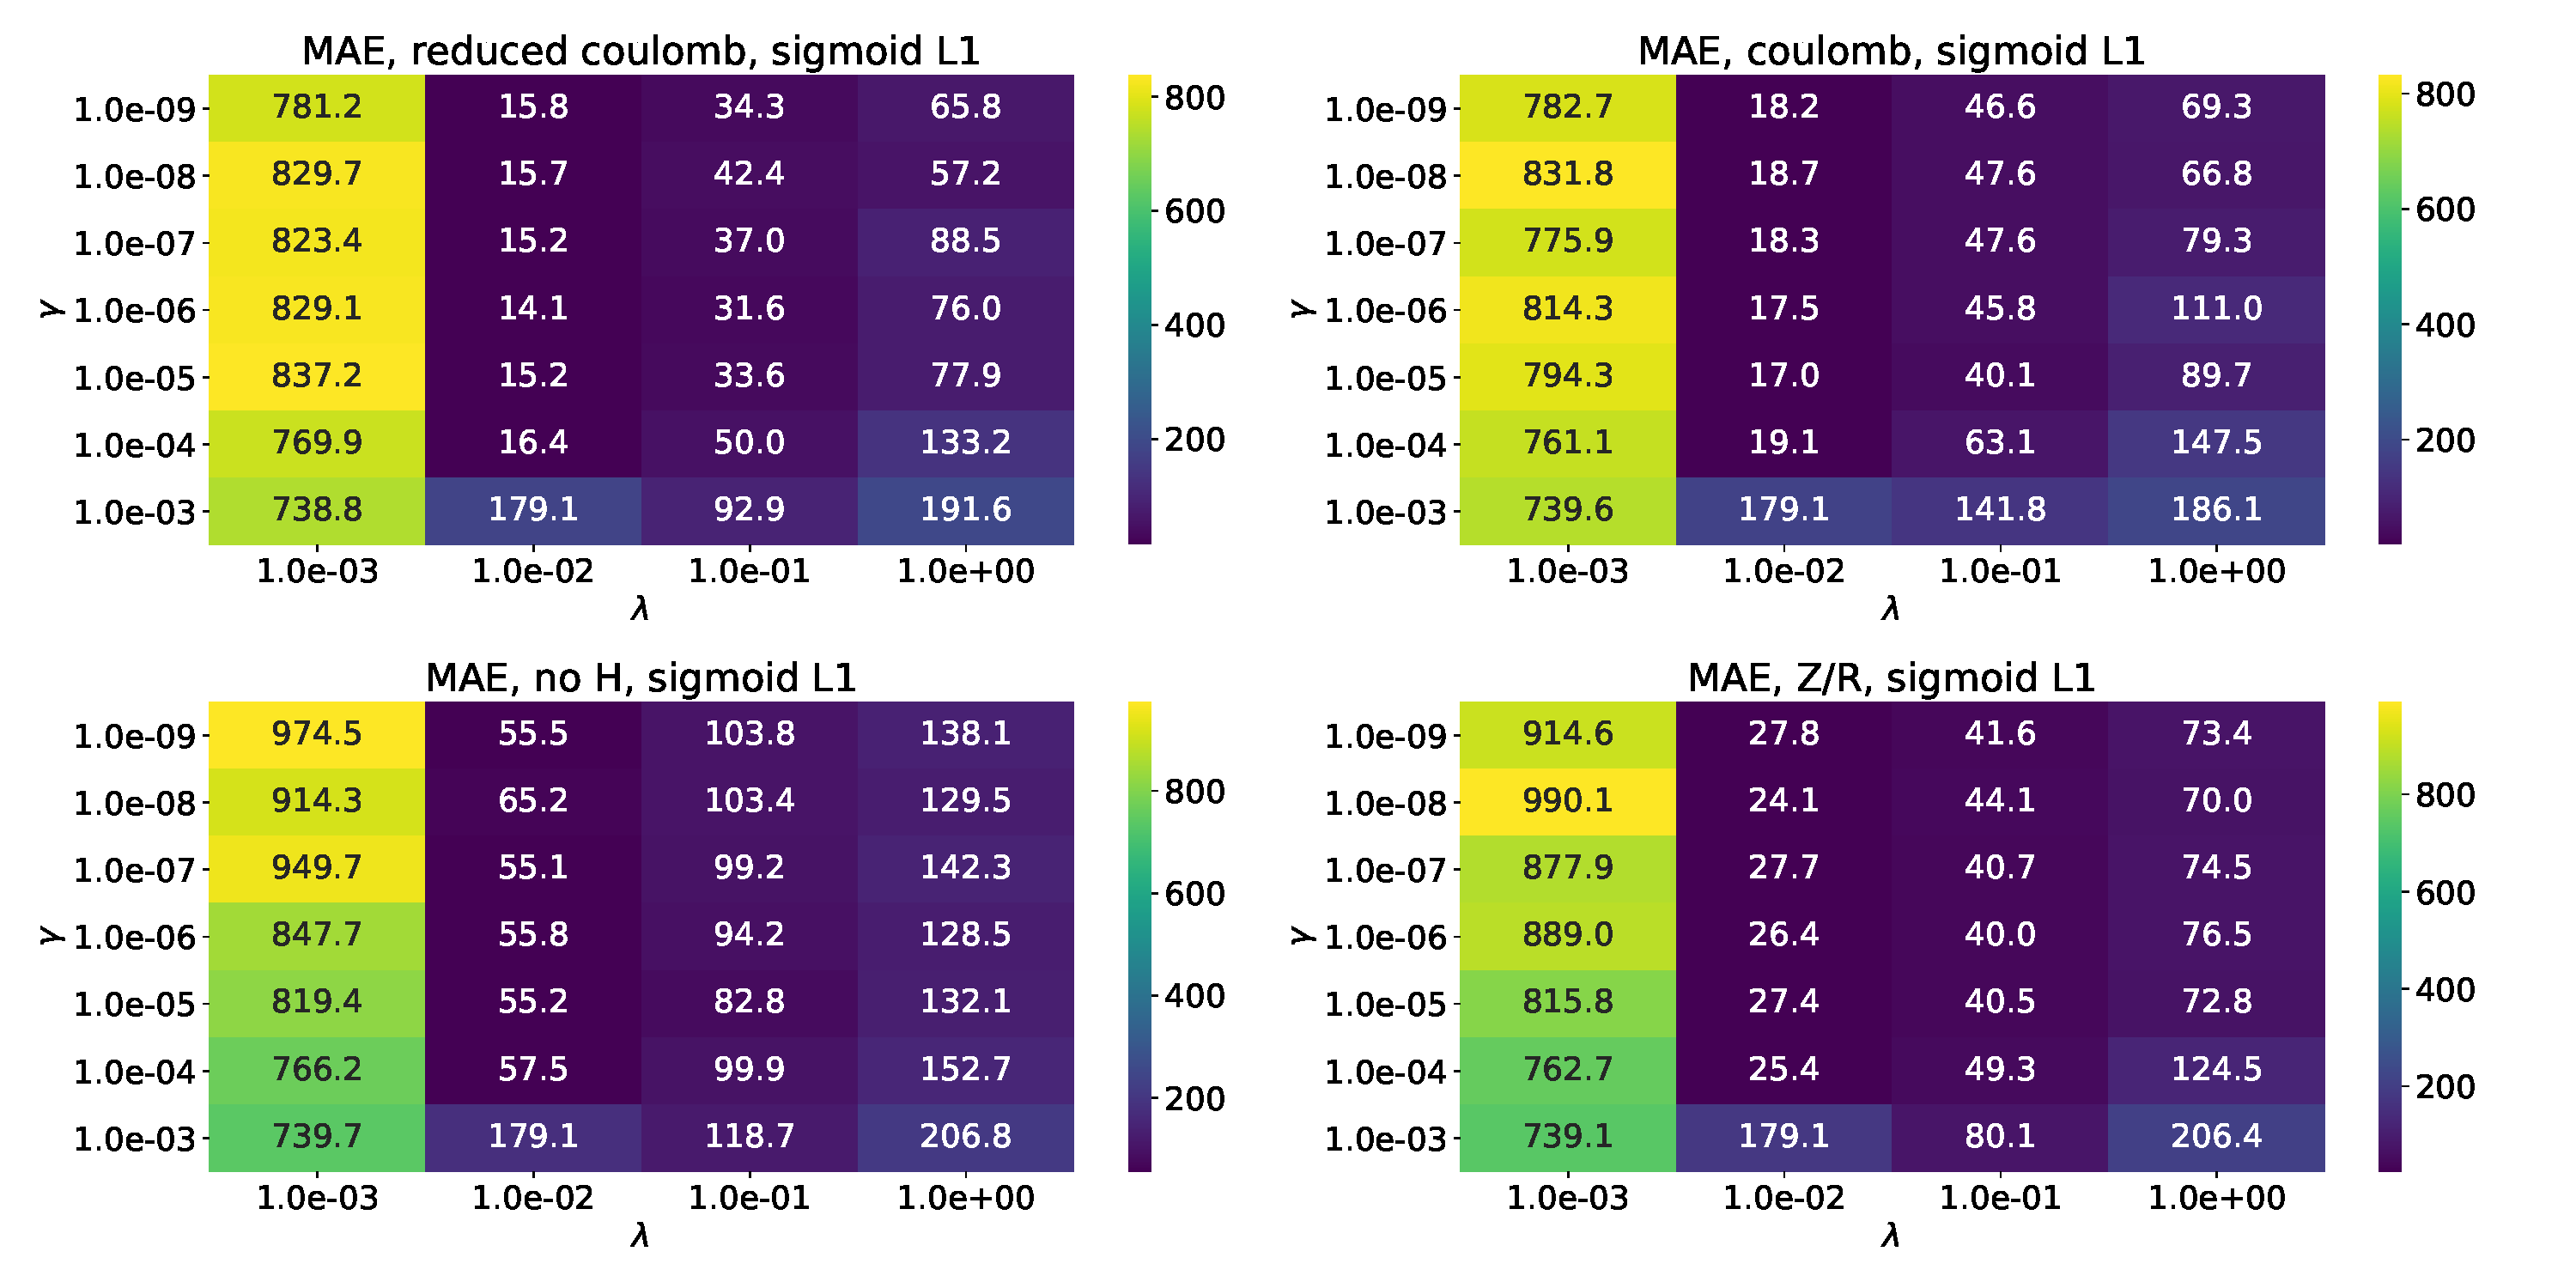
\includegraphics[width=1\textwidth]{nn_100_sigmoid L1.pdf}
\caption[NN sigmoid L1, 100 epochs]{Test MAE using the 4 different representations as function of the learning rate $\gamma$ and the regularisation rate $\lambda$ using L1 regularization and the sigmoid activation function. The Neural Network consisted of two 100-neuron layers and was trained for 100 epochs.} \label{fig:sigmoid_l1_100}
\end{figure}
\begin{figure}[H]
\centering
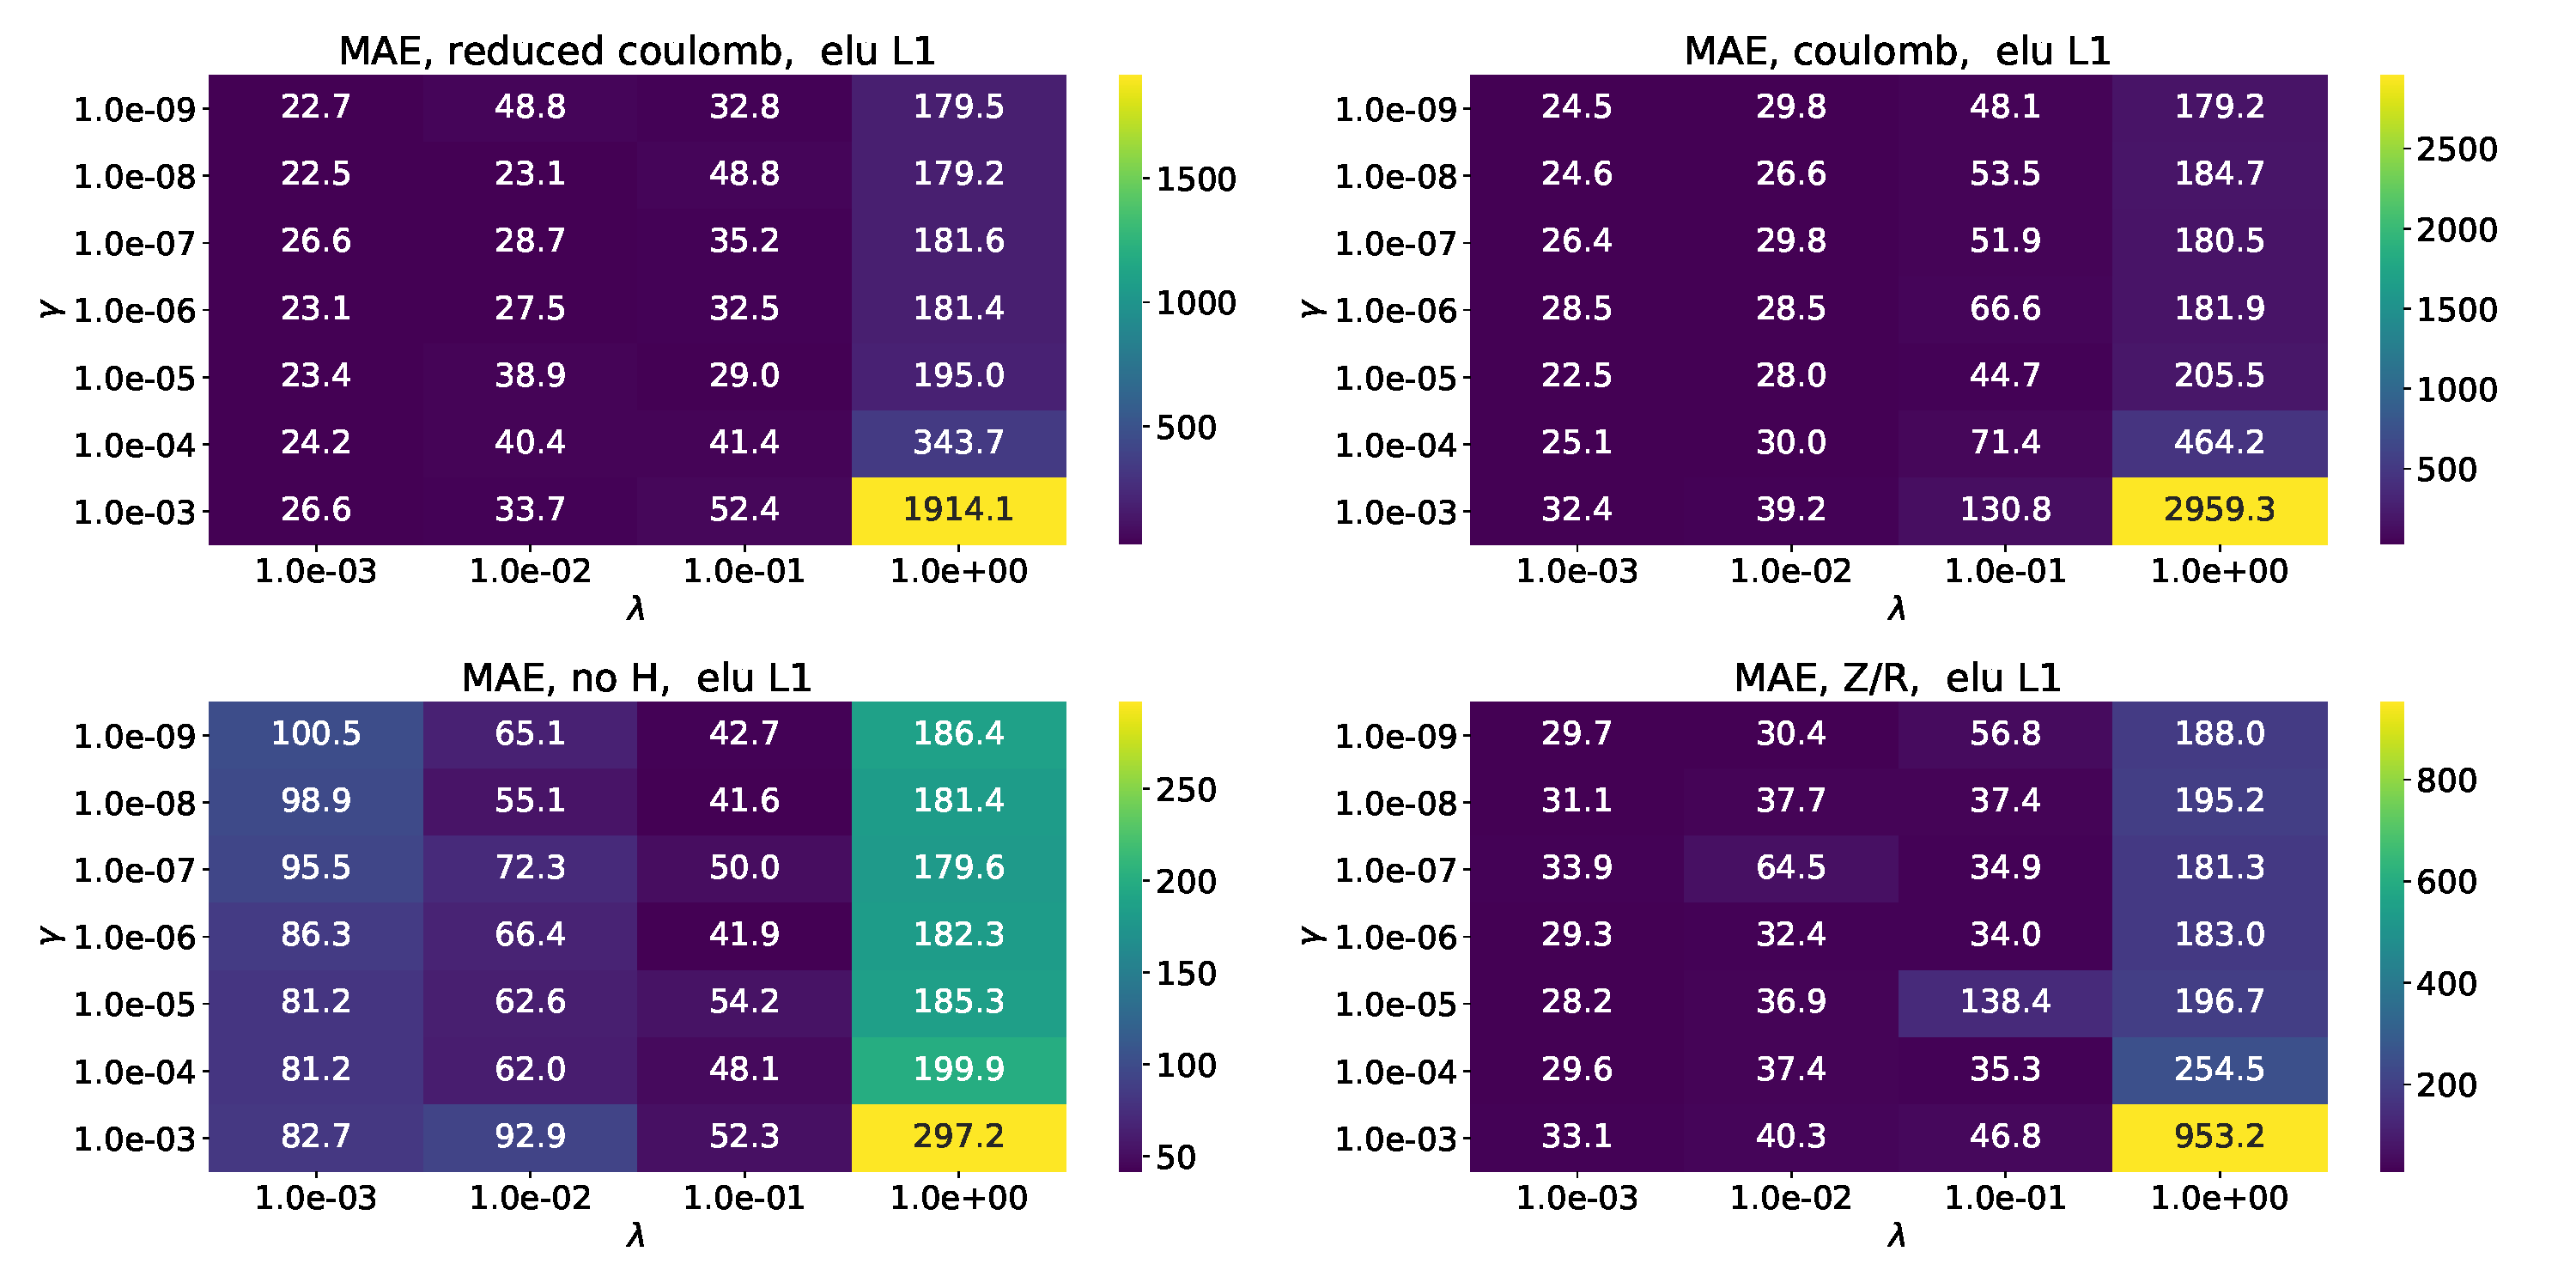
\includegraphics[width=1\textwidth]{nn_100_ elu L1.pdf}
\caption[NN elu L1, 100 epochs]{Test MAE using the 4 different representations as function of the learning rate $\gamma$ and the regularisation rate $\lambda$ using L1 regularization and the elu activation function. The Neural Network consisted of two 100-neuron layers and was trained for 100 epochs.} \label{fig:elu_l1_100}
\end{figure}
Comparing the reduced Coulomb matrices with the full Coulomb matrices and the charge-position representation, it is clear that the reduced-Coulomb matrix approach yields the best approach compared to both other representations. This matches with our expectations: The representation is unique, unlike the other two representations. As the number of parameters is smaller than for the "full" Coulomb matrix, it is also faster to use the reduced Coulomb representation. This does not prove that the other two representations, in theory, cannot give better results if they were trained differently (using a deeper Neural Network, or more epochs), but the fact that the reduced Coulomb matrix both has a theoretical justification \& yields better results for both L1 and L2 loss and both activation functions, is a strong indicator of its superiority. 
We see that the Hydrogen-free approach can yield results that get the error down to ~40 kcal/mol, which shows, when nonlinear combination of data is allowed, that a lot of information about the molecule indeed can be obtained even when Hydrogen molecules are neglected. \\
Finally, we see that the sigmoid activation function performs better than the elu activation function, for all systems but the Hydrogen-free approach. This matches our observations from \citep{Project2}, where we observed that the sigmoid function tends to be better than Linear Units for shallow Neural Networks.\\
We continued with only the reduced Coulomb representation and the hydrogen-free approach. The ideal grid-search results can be seen in table \ref{Error_table}.

\begin{table}[H]\caption[NN, Test MAE with 1000 epochs]{The test MAE using 1000 epochs in a Neural Network consisting of two 100-neuron layers. Data for the reduced Coulomb matrix and the hydrogen-free Coulomb matrix is shown. We used the elu activation function and the sigmoid activation function and both L1 and L2 regularisation. The values were obtained using a grid search in the space of the learning rate $\gamma$ and the regularization parameter $\lambda$, but it is possible that more ideal values exist outside of that range.}\label{Error_table}
\centering
\begin{tabular}{|l|l|l|l|l|}
\hline

Activation Function          & sigmoid & elu   & sigmoid & elu   \\ \hline
Regularization Type          & L1      & L1    & L2      & L2    \\ \hline
Test error (no Hydrogen)     & 35.00   & 28.66 & 35.41   & 29.48 \\ \hline
Test error (reduced Coulomb) & 12.77   & 15.18 & 14.38   & 14.71 \\ \hline
\end{tabular}
\end{table}
This shows that, when training the network longer with 1000 epochs, that it is possible to get an MAE of below 30 kcal/mol for the Hydrogen-free representation, which strengthens the observation that Hydrogens atoms only give "detailed" information. Again, we see that L1 regularization performs better than L2 regularization. Using only 1000 epochs, it is already possible to get rather good results.
\\
We continued using Neural Networks with 10,000 epochs, but got worse results than with 1000 epochs for the parameter space we have searched. This was likely due to overfitting caused by badly chosen parameters. We did not continue trying to look for better results due to the high learning time and the lack of opportunity to use GPU-accelerated TensorFlow. According to the \href{http://quantum-machine.org/datasets/}{quantum-machine} web page, they managed to get the MAE down to 3-4 kcal/mol with a simple two-layer Neural Network. However, the code they provide gives error messages and the Neural Networks trains for 1,000,000 epochs, which would take several days. For this reason, we can neither confirm or deny these results. However, we can compare our analysis to \citep{Atomization_network}. They used a Bayesian Regularized Neural Network using the same type of reduced Coulomb matrix and managed to get a test MAE of 4.4 kcal/mol. They also created a set of predictors that combines the  reduced Coulomb matrix with the charge-position representation. This way, they managed to get the test MAE down to 3.0 kcal/mol.
\subsection{Ridge Regression and PCA}
Figure  \ref{fig:Variance} shows the  total cumulative variance  as function of the percentage of included Principal Components for the reduced Coulomb matrix, as well as the reduced Coulomb matrix after the removal of all hydrogen atoms. Figure \ref{fig:Errors_PCA_ridge} shows the test and train Mean Absolute errors using Ridge Regression (with the ideal regularization parameter $\lambda$) as function of the number of used Principal Components. 


\begin{figure}[H]
\centering
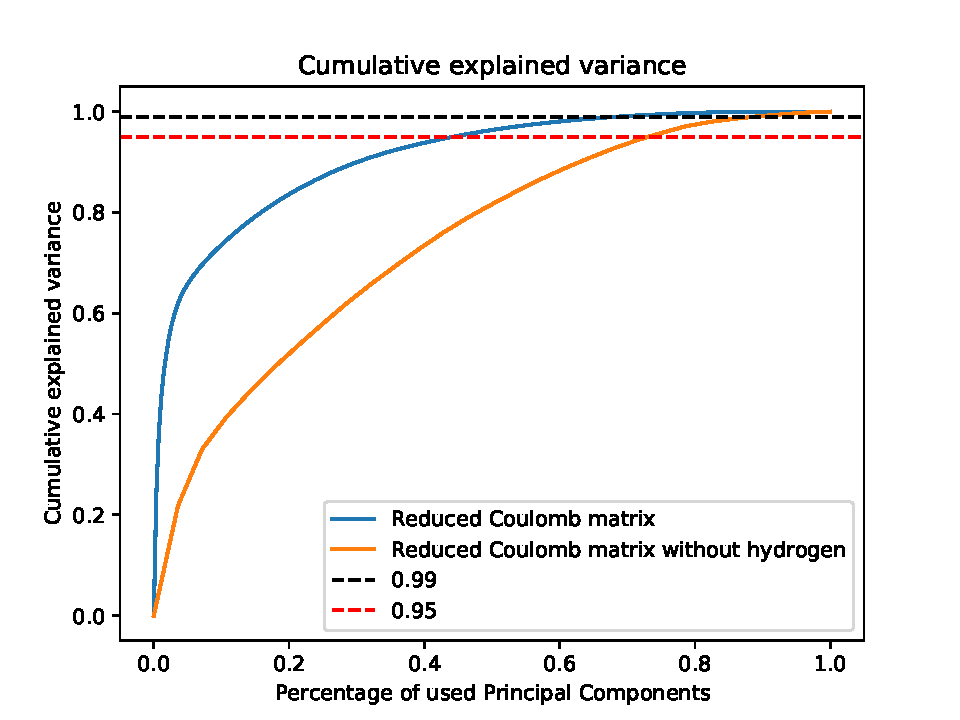
\includegraphics[width=0.8\textwidth]{Cumulative_variance.pdf}
\caption[Cumulative Explained Variance]{Cumulative explained Variance as function of the Percentage of used Principal Components (ordered). There are 276 PCs for the reduced Coulomb matrix, while there are 28 Principal Components for the hydrogen-free variant. Horizontal lines were added to indicate the threshold for 95\% and 99\% explained variance.} \label{fig:Variance}
\end{figure}
\begin{figure}[H]
\centering
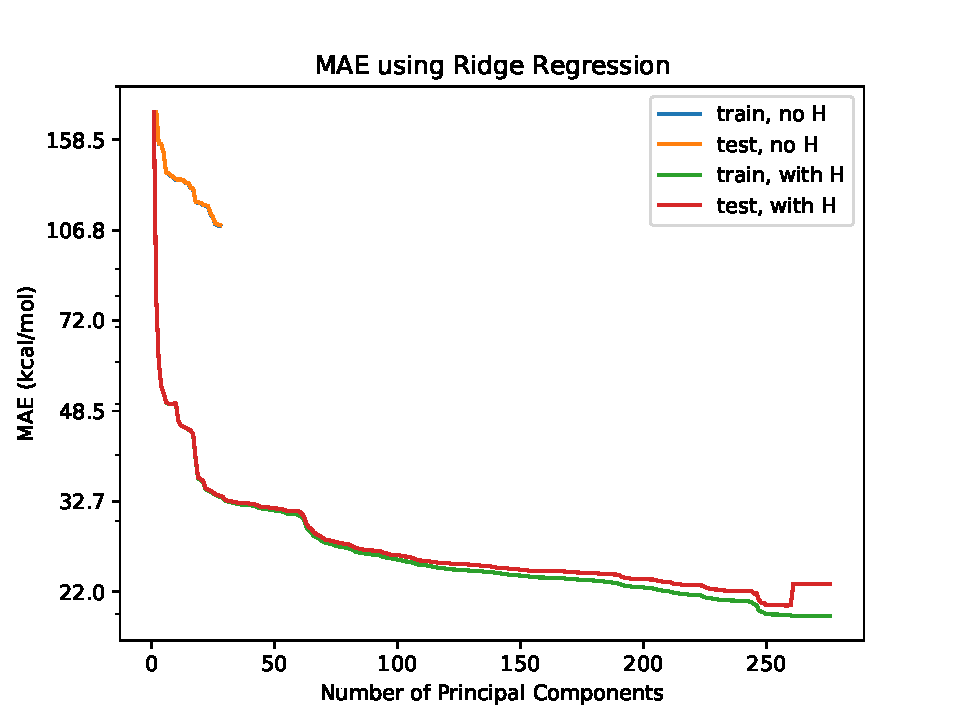
\includegraphics[width=0.8\textwidth]{Ridge_error.pdf}
\caption[Ridge Error]{MAE using Ridge Regression as function of number of used Principal Components (ordered). There are 276 PCs for the reduced Coulomb matrix (with h), while there are 28 Principal Components for the hydrogen-free variant (no H). Both test and train error for both approaches were included} \label{fig:Errors_PCA_ridge}
\end{figure}

We see that the removing hydrogen atoms does not give good results and is completely qualitative when using Ridge Regression, with an MAE above 100 (109 for both testing and training) even when the full Design Matrix (all Principal Components) is used. This is to be compared to the MAE of 33 using 28 PCs of the full reduced Coulomb matrix.  This does not necessarily mean that the predictors are bad, as we have seen with Neural Networks, but it shows that the linear approach does not suffice here. One could for example include higher-order terms. However, using a Multivariate Vandermonde-type matrix with 28 variables becomes very large for polynomial degrees larger than 2, and from the fact that the Design matrix containing hydrogen atoms performs so much better, it seems rather improbable that these results would be on pair with the full reduced Coulomb matrix. \\
However, we also see that removing hydrogen atoms has some advantages. In the full reduced Coulomb matrix, there are 15 dependent Principal Components, which increase the test error when included, and don't explain any variance in the data. This is not the case with the hydrogen-removed reduced Coulomb case, which shows that there are some linear dependencies when Hydrogen is included. From the Cumulative explained variance curves, we can also see that the hydrogen-free curve raises steeper, which shows that the same percentage of the used Principal Components explains less of the data, which also shows that the vectors in the Hydrogen-free approach are further away from singularity. \\
In the approach were full reduced Coulomb matrices are used, we see that using only 10 PCs, it is possible to get the test error down to 50 kcal/mol. However, it is also clear that the error keeps decreasing when more PCs are being used, and the MAE goes down to 20.75 kcal/mol at 259 PCs with a train error slightly below 20 kcal/mol. This shows that all Principal Components need to be used in order to use the data quantitatively, as the error is more than halved between 10 PCs and the full set of PCs. It is also interesting to see that there is a large "jump" at around 60 PCs, which shows that some less important Principal Components lead to comparatively strong improvements.\\

This approach using Ridge Regression on the reduced Coulomb matrix should be compared to \citep{Atomization_Ridge}. There, the authors used Kernel Ridge Regression with Gaussian functions as Kernels, and they do not use the linear parameters of the Coulomb matrix like is done here, but rather the dissimilarity between two molecules which is calculated from the eigenvalues of the Coulomb matrix. This approach yields dedicedly better results, with a test MAE of ~10kcal/mol.

\subsection{Decision Trees}
We implemented a simple decision tree to fit the data. Figure \ref{fig:Decisiontree} contains the test and train MAE as function of the maximal tree depth. Errors were obtained using 5-fold Cross Validation.
\begin{figure}[H]
\centering
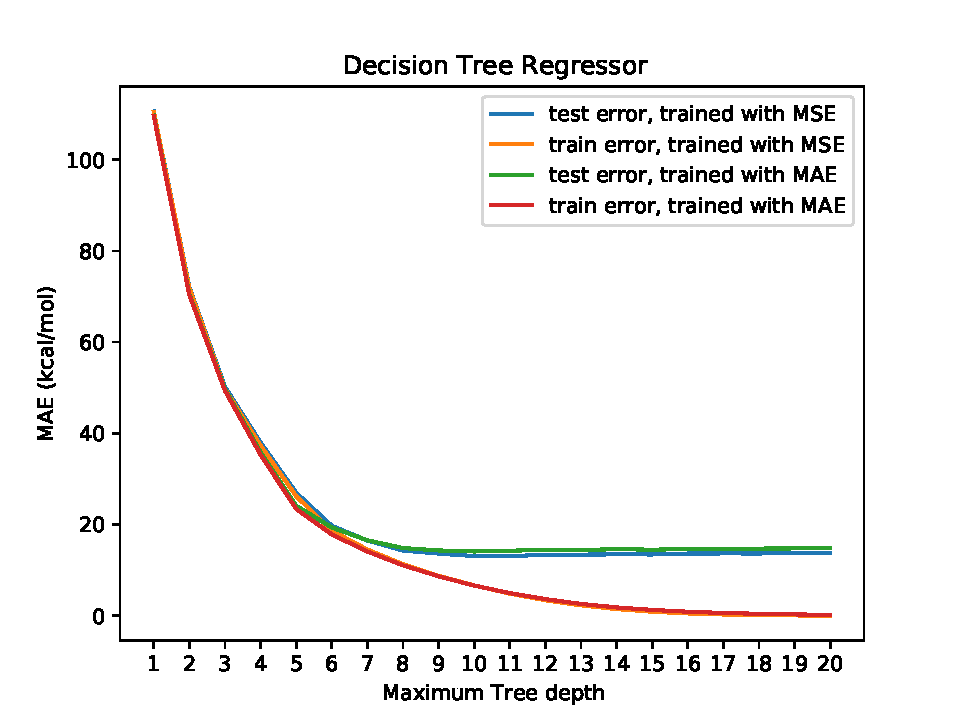
\includegraphics[width=0.8\textwidth]{decision_tree.pdf}
\caption[Decision Tree]{Test and Train MAE using 5-fold Cross-Validation for a Decision Tree, using the CART algorithm to minimize either MSE or MAE, as function of the maximum tree depth.} \label{fig:Decisiontree}
\end{figure}
The results were surprising, as we did not expect a simple Decision Tree to perform that well. When reducing the MAE, we found an ideal test MAE of 14.10 kcal/mol at a maximum depth of 9, while we found that, when reducing the MSE, we found an ideal test MAE of 13.05 kcal/mol at a maximum tree depth of 10. The train MAE is slightly better for the MAE-trained version, but does not improve the test error. Due to the much higher time usage of the MAE method and the fact that it gave worse results, we decided to only use the CART algorithm for MSE for bagging, random forests and boosting. \\

The fact that there is only a slight overfitting as the tree depth is increased beyond the ideal value shows that estimating molecular energies works surprisingly well by simply finding the molecule which is "the most similar", which is what overfitting Decision Trees do. The fact that this clearly beats Ridge Regression comes as a big surprise. \\

We also implemented a Decision Tree for the Hydrogen-free approach. This is shown in figure \ref{fig:decisiontreenoH} in the appendix. The results clearly beat those attained using Ridge Regression, but a test MAE of 80 kcal/mol is still too large to do any useful predictions.  
\subsection{Bagging with Decision Trees}
We implemented Bagging using a simple decision tree as weak learner. Figure  \ref{fig:bagging_1}  plots the 5-fold Cross Validation MAE as function of the number of Trees used (which is the same as the number of bootstraps). Here, we used trees of max depth 20, using the same number of samples as there are in the data set. This approach reduced the test MAE further, down to 10.20 kcal/mol when using 1000 trees. Here, the train error does not approach zero, which is an indicator that overfitting is being avoided to a higher degree, but we also see that the test error stops increasing. We also used smaller trees (with a maximum depth of 7 and maximum 1000 samples) and up to 10,000 bootstraps, which gave an ideal test MSE of 15.96 kcal/mol at 3162 trees. This is shown in figure \ref{fig:bagging_2} in the appendix. This shows that using deep trees that train on a lot of data is a good idea for Bagging in this case.
\begin{figure}[H]
\centering
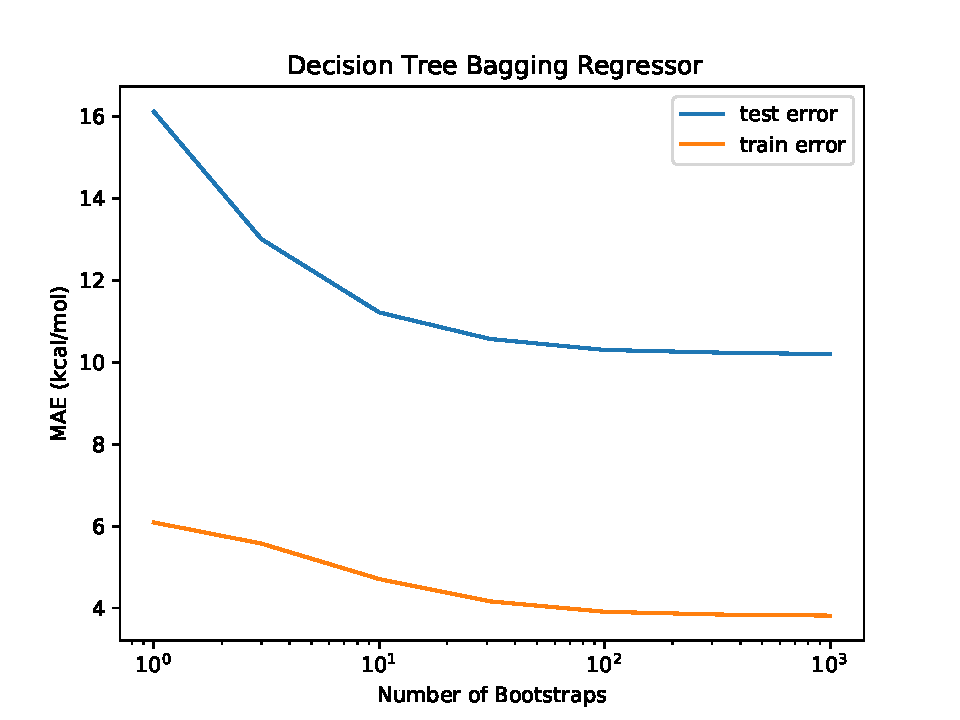
\includegraphics[width=0.8\textwidth]{bagging.pdf}
\caption[Bagging]{Test and Train MAE using 5-fold Cross-Validation for Bagging as function of the number of Trees grown with Decision Trees as weak Learners, where we used trees of max depth 20, using the same number of samples as there are in the data set. The CART algorithm was used to minimize the MSE for each tree.} \label{fig:bagging_1}
\end{figure}

 We see that Bagging gives better results than Decision Trees, but they lack the simple interpretability of a single Decision Tree. 
 
 We also implemented Bagging for the Hydrogen-free approach. This is shown in figure \label{fig:baggingnoH} in the appendix. The test MAE improves to approximately 50-60 kcal/mol. 

\subsection{Random Forests}
We implemented Random Forests with 25, 9 and 5 trees and used either the whole set of predictors for each tree (which is the same as bagging), or only the square root of predictors, or a third of all predictors, as recommended in \citep{hastie} for Regression. We plotted the number of trees against the 5-fold Cross Validation MAE. This is shown in figure \ref{fig:What_about_the_forests?}.
\begin{figure}[H]
\centering
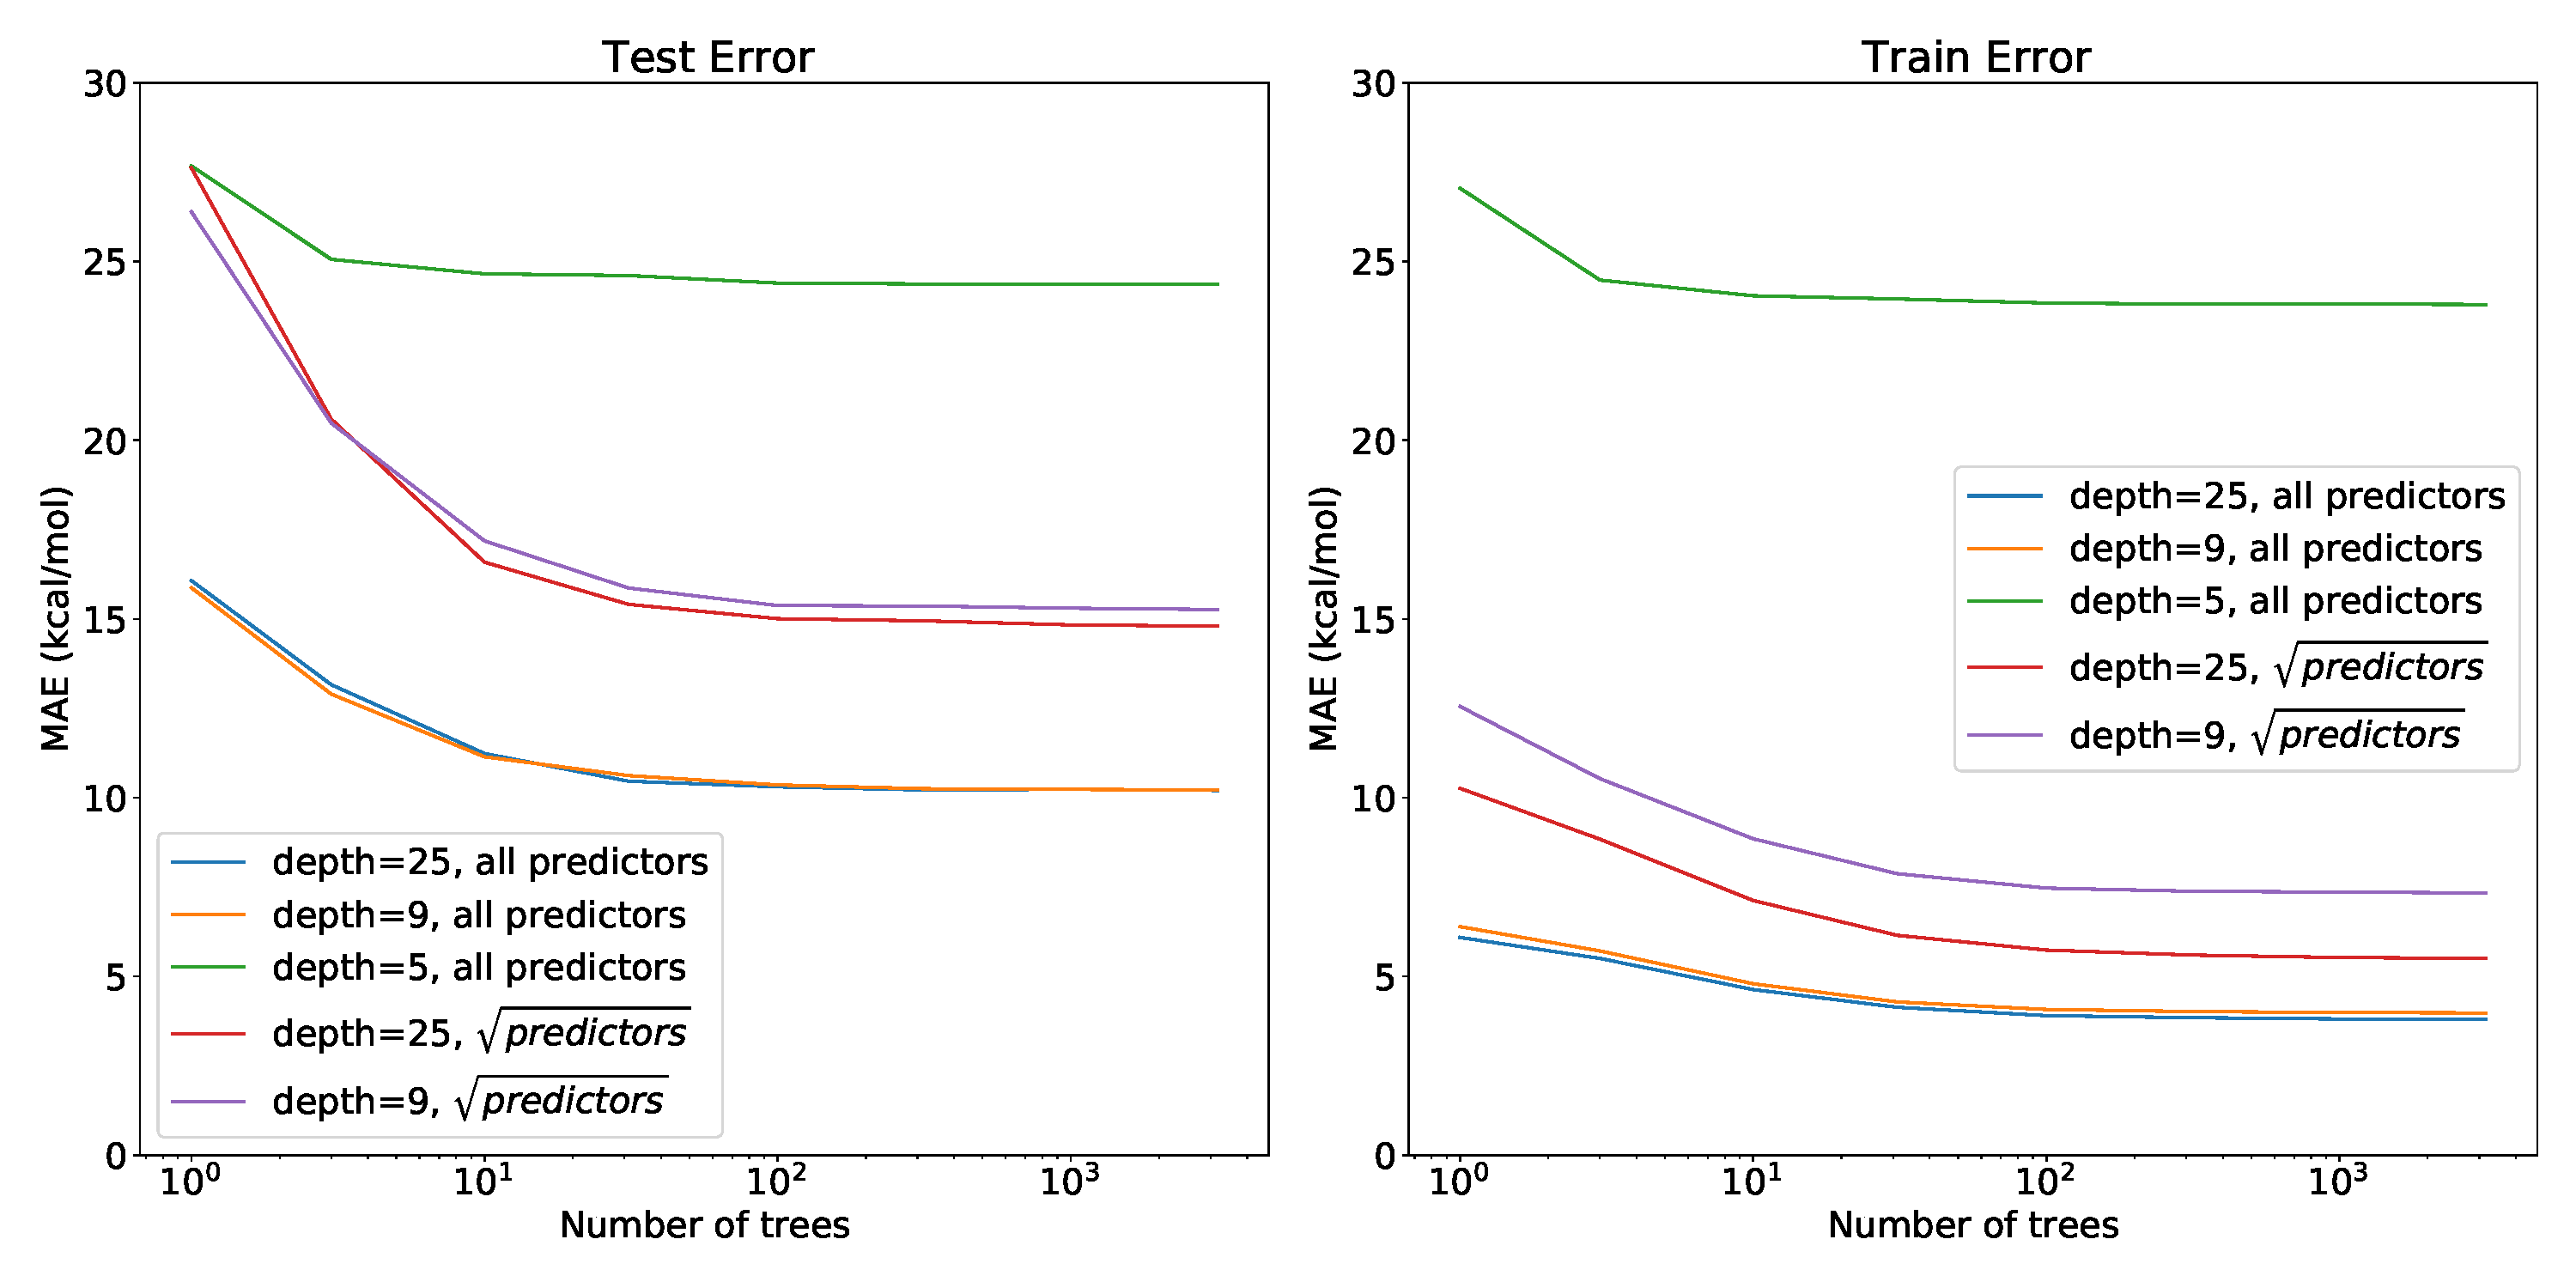
\includegraphics[width=1\textwidth]{forest.pdf}
\caption[Random Forest]{Test and Train MAE using 5-fold Cross-Validation for Random Forests as function of the number of Trees grown with Decision Trees as weak Learners, where we used trees of different max depths with different numbers of predictors being used. The CART algorithm was used to minimize the MSE for each tree.} \label{fig:What_about_the_forests?}
\end{figure}
The minimum test error is attained using a tree depth of 25 and all predictors (that is, bagging) and $10^{3.5}$ trees, with MAE=10.21 kcal/mol. This is more or less the same result as for bagging. As we can see in the graph, whether we use a max depth of 9 of 25 makes almost no difference when all predictors are used, but it does when only the square root of all predictors are being used. Using only the square root of all predictors is not recommended for Regression anyways, and this recommendation holds for our data set, too. We see that using fully grown trees gives much better results than shorter trees, and using more trees improves the results, however, the difference between $10^{3.5}$ and $10^{3}$ trees is marginal and the improvement eventually stops.

 We also implemented Random Forests for the Hydrogen-free approach. This is shown in figure \ref{fig:randomforestnoH} in the appendix. The MAE improves to approximately 50-60 kcal/mol. The overall analysis is more or less identical to the full data set, however we observe that deeper trees are required in order to get the optimal test error.

\subsection{Boosting}
As Boosting has a large number of parameters, we decided to rely on the description in \citep{hastie}, which states that it is generally worthwhile to use small learning rates $\eta$ and correspondingly larger values of the number of learners M, we plotted the number the MAE as function of the number of learners M, where we kept $M\eta=50$ for different tree depths. This can be seen in figure \ref{fig:boosting1}.
\begin{figure}[H]
\centering
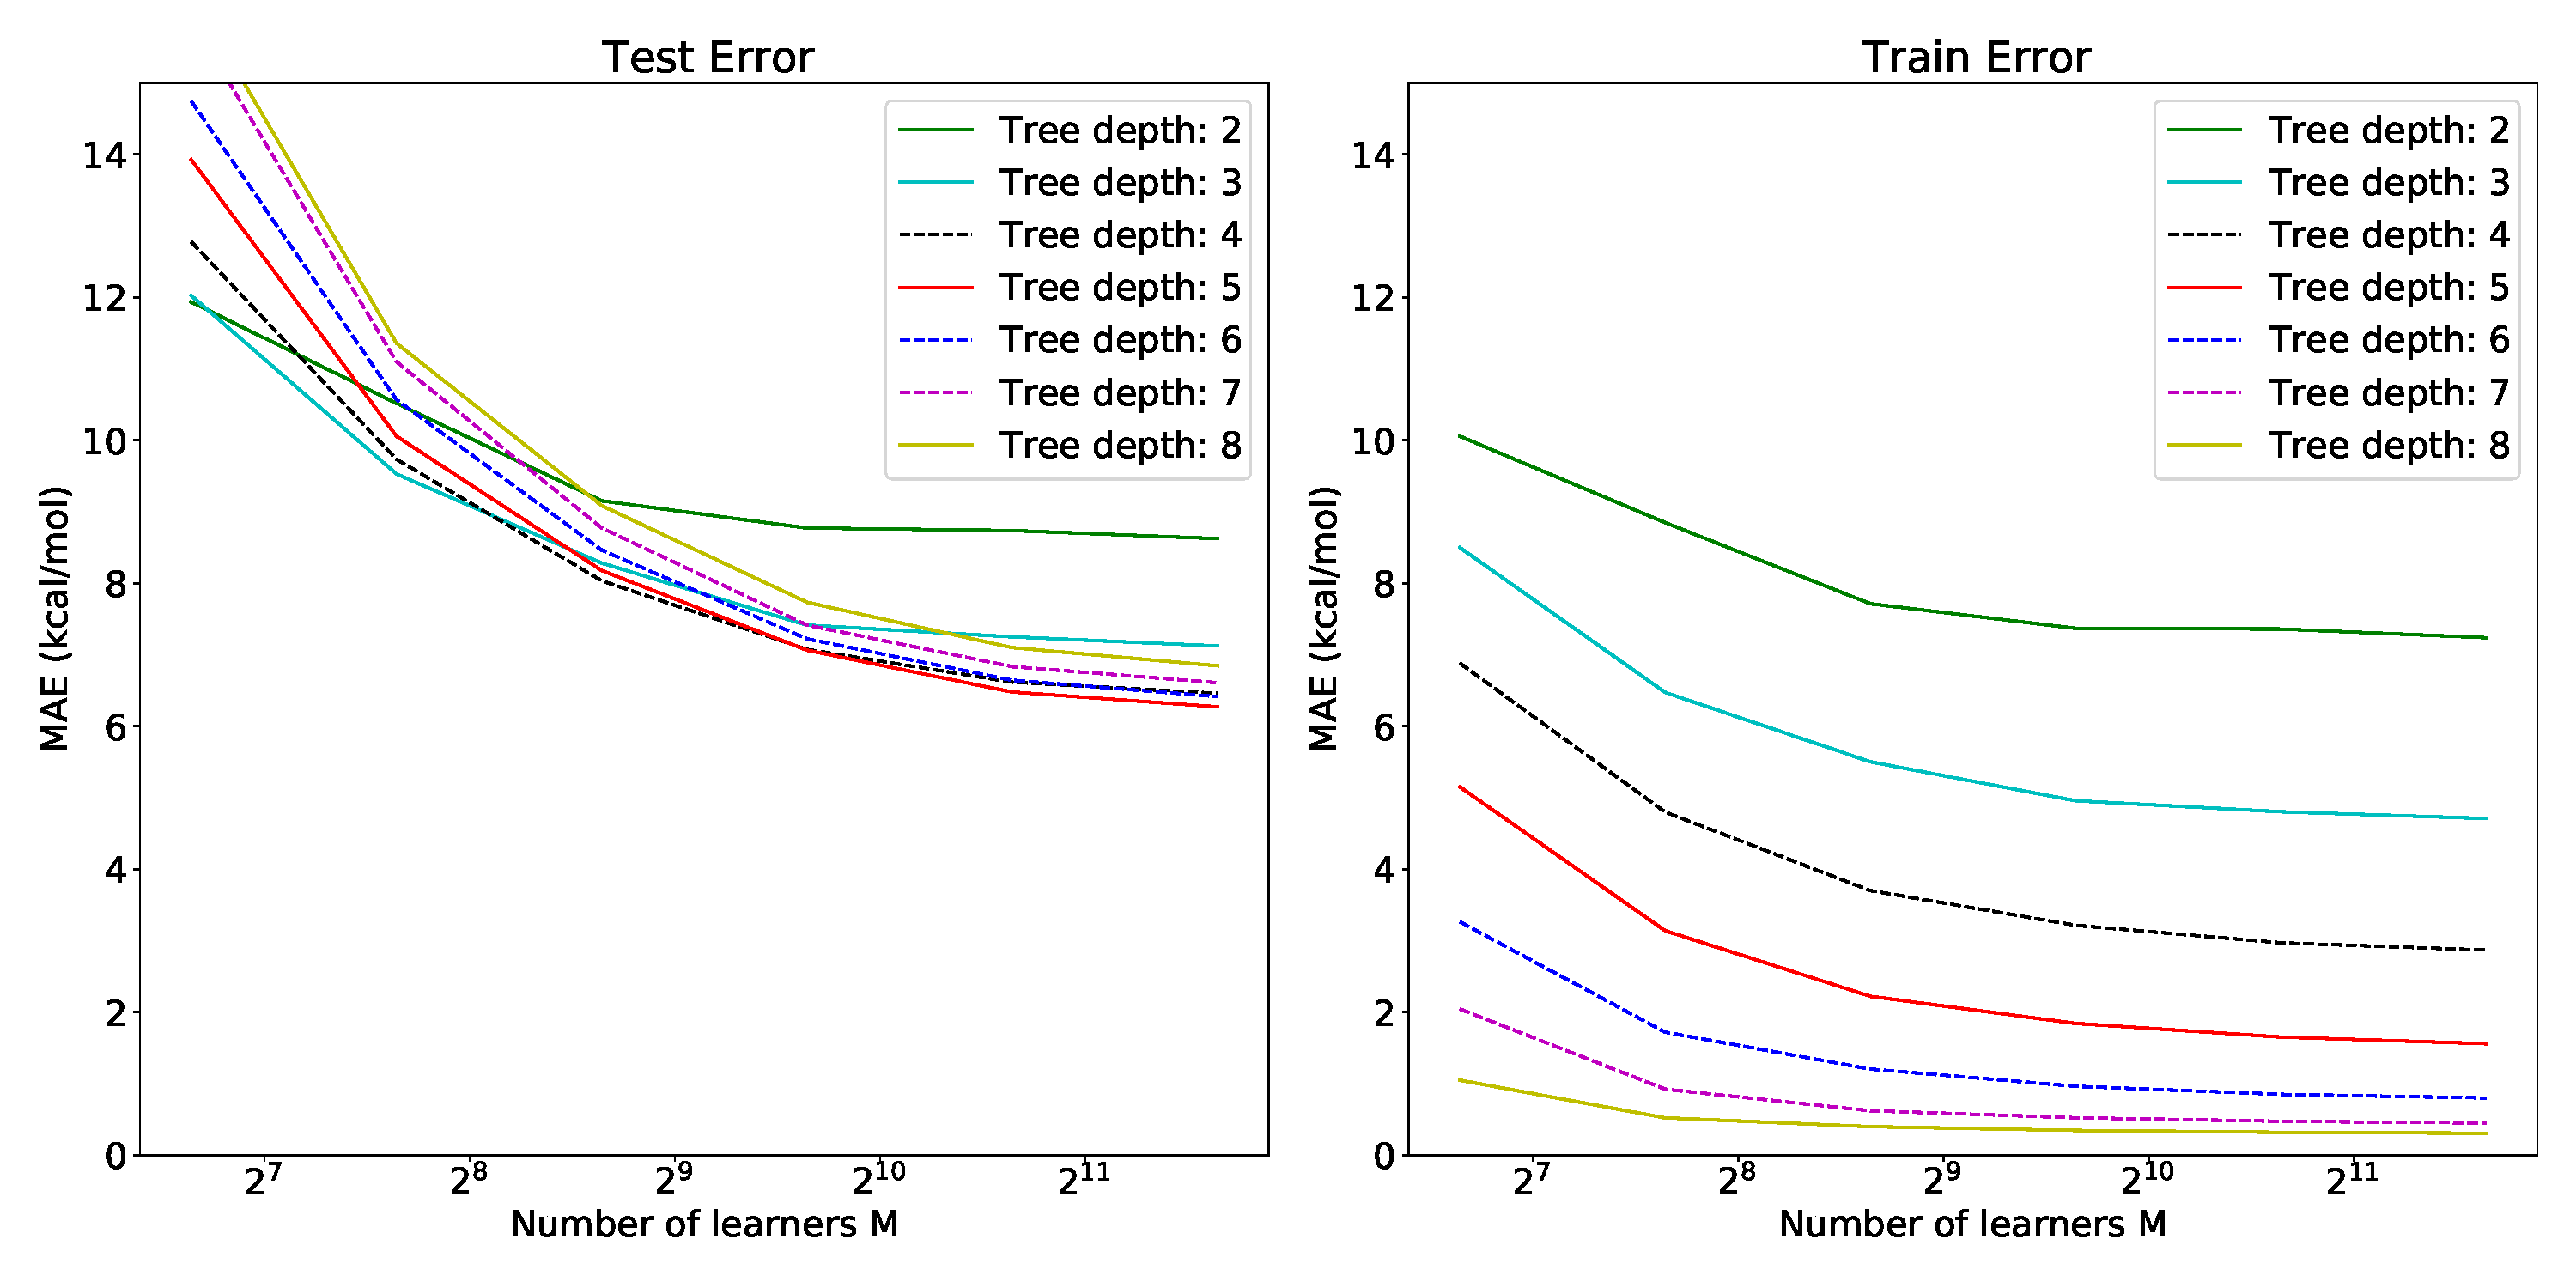
\includegraphics[width=1\textwidth]{boosting1.pdf}
\caption[Boosting $M\eta=50$]{Test and Train MAE using 5-fold Cross-Validation for Boosting as function of the number of Trees grown with Decision Trees as weak Learners, where we used trees with variable maximum depth (see label). We used a L1 regularisation of $\lambda_{L1}=10$, sampled 50\% of samples and 30\% of features, and adapted the learning rate $\eta=50/M$} \label{fig:boosting1}.
\end{figure}
We see that the largest M with the smallest learning rate generally gives the smallest test error. We also see that a tree depth of 4-8 generally gives similar results, as stated in \citep{hastie}. We get the impression that 5 works best here and will continue using that value. Finally, we see that boosting works really well and we get MAE slightly above 6 kcal/mol.\\\\
We ran a similar simulation as the one shown in figure \ref{fig:boosting1} for the Hydrogen-Free approach. This is shown in figure \ref{fig:boosting3} in the appendix. We see that a tree depth of 6 works best here, and we  got the MAE down to 27.48 kcal/mol.

In figure \ref{fig:boosting2}, we plot again the learning rate as the number of learners M, this time keeping the learning rate fixed at respectively 0.01 and 0.05, for different regularization rates $\lambda_{L1}$.
\begin{figure}[H]
\centering
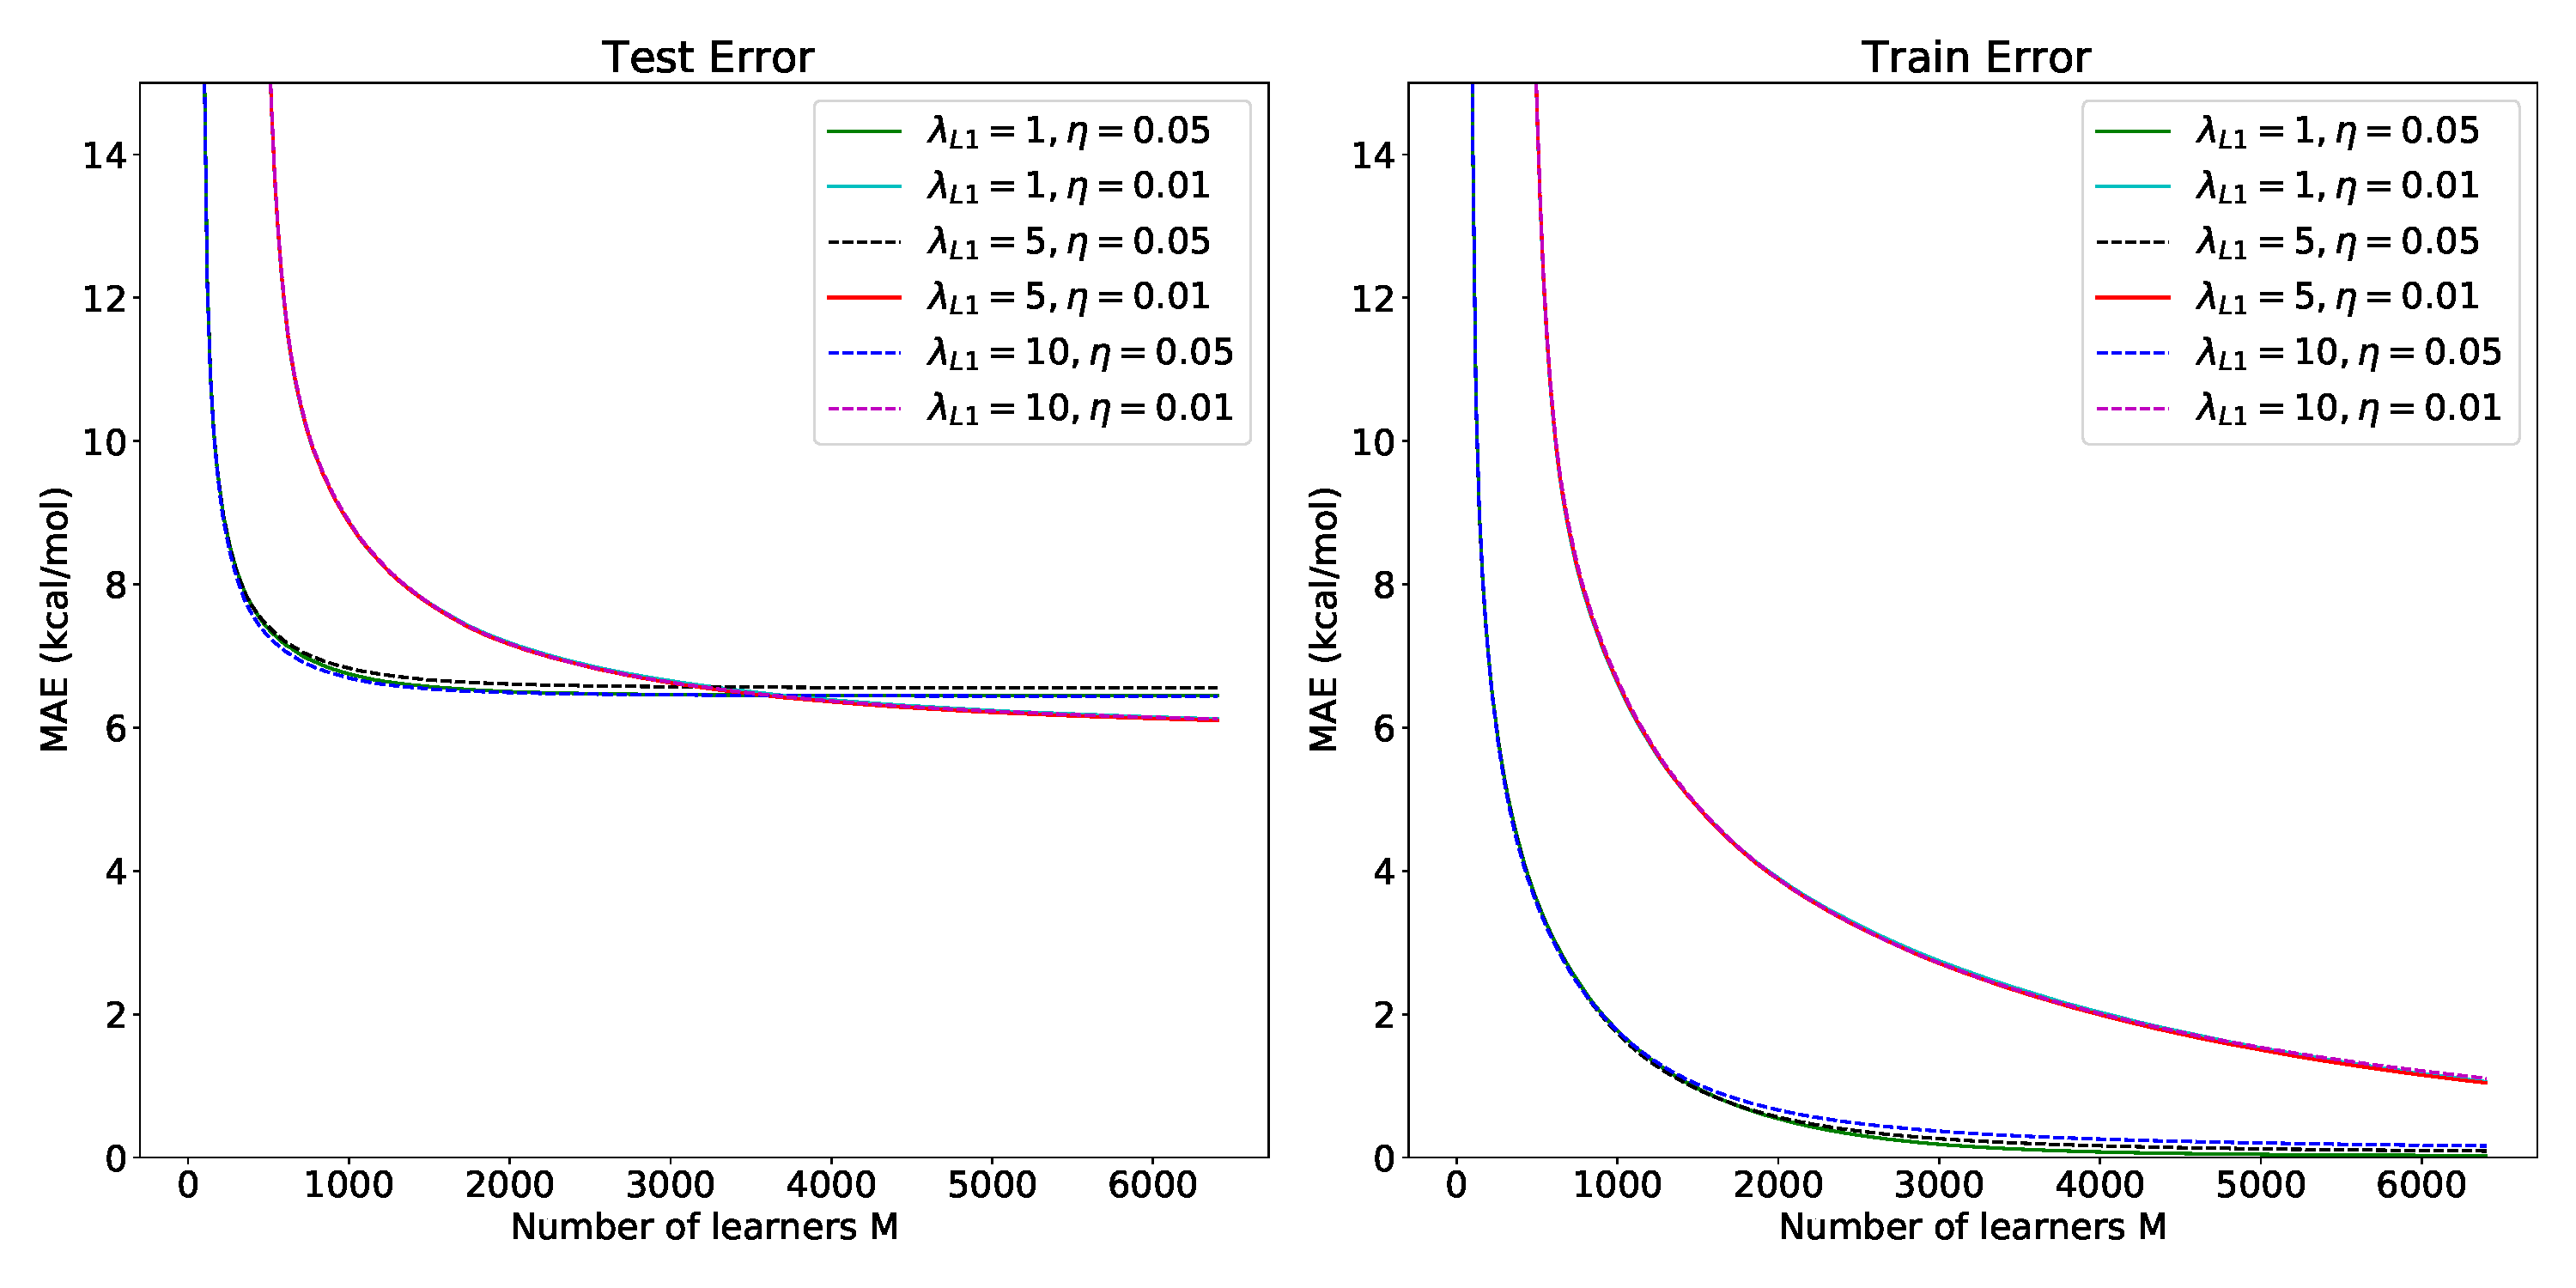
\includegraphics[width=1\textwidth]{boosting2.pdf}
\caption[Boosting $M,\lambda_{L1}$]{Test and Train MAE using 5-fold Cross-Validation for Boosting as function of the number of Trees grown with Decision Trees as weak Learners, where we used trees with variable maximum depth (see label). We used different L1 regularisation parameters  $\lambda_{L1}$, sampled 50\% of samples and 30\% of features, and tested for different learning rates $\eta$.} \label{fig:boosting2}.
\end{figure}
We can see that the choice of $\lambda_{L1}$ has neglecting effects, but choosing a lower learning rate leads to less overfitting, which we suppose leads to the "stop" in increasing test accuracy for the larger learning rate. Training got increasingly slower, that why we stopped after 6400 steps. With $\lambda_{L1}=5$ and $\eta=0.01$, we got a Cross-Validation MAE of 6.10  kcal/mol. 
\\
We also used some of the advanced features of XGboost, using the histogram optimized approximate greedy algorithm $gpu\_hist$ and a sampling algorithm where the selection probability depends on the absolute value of the gradient \citep{XGboost}. This way, we trained with M=20,000 for $\lambda_{L1}=5$ and $\eta=0.01$ and got a Cross-Validation MAE of 6.07  kcal/mol, even though we assume that optimized parameters and longer training might reduce that value even further. \\

\section{Conclusion}
In this article, the aim was to compare different algorithms and different representations of the data set to predict the atomization energies of molecules. We started by analysing, using Neural Networks, which representation of Neural Network that gives the best results for predicting atomization energies, and found that, as is theoretically founded, the reduced Density matrix works best of all approaches. With Neural Networks, we managed to get an $MAE \approx 13$ kcal/mol, even though we suppose that, when training very long and using ideal parameters, that it is possible to cut that value in half. We then went and explored the PCA of the reduced Density matrix and the reduced density matrix without hydrogen atoms using Ridge Regression and found that the data is not dominated by few Principal Components, but rather that most Principal Components are important, even though there are linear dependencies when Hydrogen is included. We also found that Ridge Regression is not a suitable method compared to the other methods, with  $MAE>20$ kcal/mol. We were surprised by the goodness of the fit of a single Decision Tree, which managed to give us an  $MAE \approx 13$ kcal/mol, too, by using a maximum tree depth of 10 trees. We continued and explored ensemble methods (Bagging and Random Forests) and got an $MAE \approx 10$ kcal/mol with Bagging and a large number of deep (depth=25) trees. Finally, we managed to get an $MAE = 6.07$ kcal/mol using Boosting with small learning rates and a complex model (M=20,000), and we think that lower values are still possible. While this is not chemical precision ($MAE < 1$ kcal/mol), it is on pair with what many quantum chemical simulations need much longer time for (after the network is trained). \\ Finally, we found that, for representations where Hydrogen is cut out, that Ridge Regression (linear in the parameters of the reduced density matrix) gives very bad results $MAE > 100$ kcal/mol, while it gives decent results for Neural networks  $MAE < 30$ kcal/mol and Boosting  $MAE \approx 13$ kcal/mol, showing that qualitative predictions are possible without hydrogen atoms, but not quantitative onesf. \\

All methods have their advantages and disadvantages. Decision Trees gives very explainable results, and so does Ridge Regression, but these two methods also gave worse results than the other methods. For Ridge Regression, we see that Kernel Ridge Regression and parameters that are not identical to the Coulomb-matrix representation, cut our error in half \citep{Atomization_Ridge}. However, the fact that a Single Decision tree performed as good as a (really badly) trained Neural Network, was a positive surprise for us, which shows that simple Decision-based approaches might be a good descriptor of chemical attributes. \\Ensembles of trees lack the easy explainability of Single Trees, but the idea of averaging over many different trees is still less abstract as what happens in Neural Networks or Boosting and relatively easy to implement. \\ Neural Networks and Boosting are both very strong Machine Learning algorithms that can give very good results, however, we did not manage to find good parameters for the Neural Network and got results inferior to ensembles of trees, even though we think that much better results are absolutely obtainable (see the earlier stated claim on the \href{http://quantum-machine.org/datasets/}{quantum-machine} web page). Boosting worked really well for us and we managed to get an MAE which is only $\approx1.5$ kcal/mol higher than the value achieved in $\citep{Atomization_network}$ with the same dataset. However, both Boosting and especially Neural Networks have a plethora of parameters to fix, both have long training times, and the results are difficult to interpret. Personally, we think that the adaptive learning of Boosting is very intriguing, and it seems easier to get good (but by no means ideal) results without tweaking very many parameters and too long training time, compared to Neural Networks.\\

In this article, we only looked very superficially at many of the Machine Learning algorithms and libraries. Especially TensorFlow and XGboost have extremely many parameters to tweak, which we did not explore. Deeper analysis of these functionalities might give better results than those we have achieved. This also holds for the  Decision-Tree based approaches, we did not delve into options such as Tree Pruning \citep{MortenLectureNotes}. These are some ways to improve upon our results. \\
The dataset is not very big, and it is likely that larger data sets will give even better results. We only explored some of the possible representations of molecules, but it might be possible to find even smarter predictors, such as the combination of Coulomb matrices and R/Z representation \citep{Atomization_network}. It is also possible to "expand" the dataset by reordering the Coulomb matrices (the same molecule), increasing the number of samples. Here, we used atomization energy as target, but really, any chemical property could be used as target. The here described methods can be used for that data, too, obtaining either better results or additional information. 
\section{Appendix}
\subsection{Figures}
\begin{figure}[H]
\centering
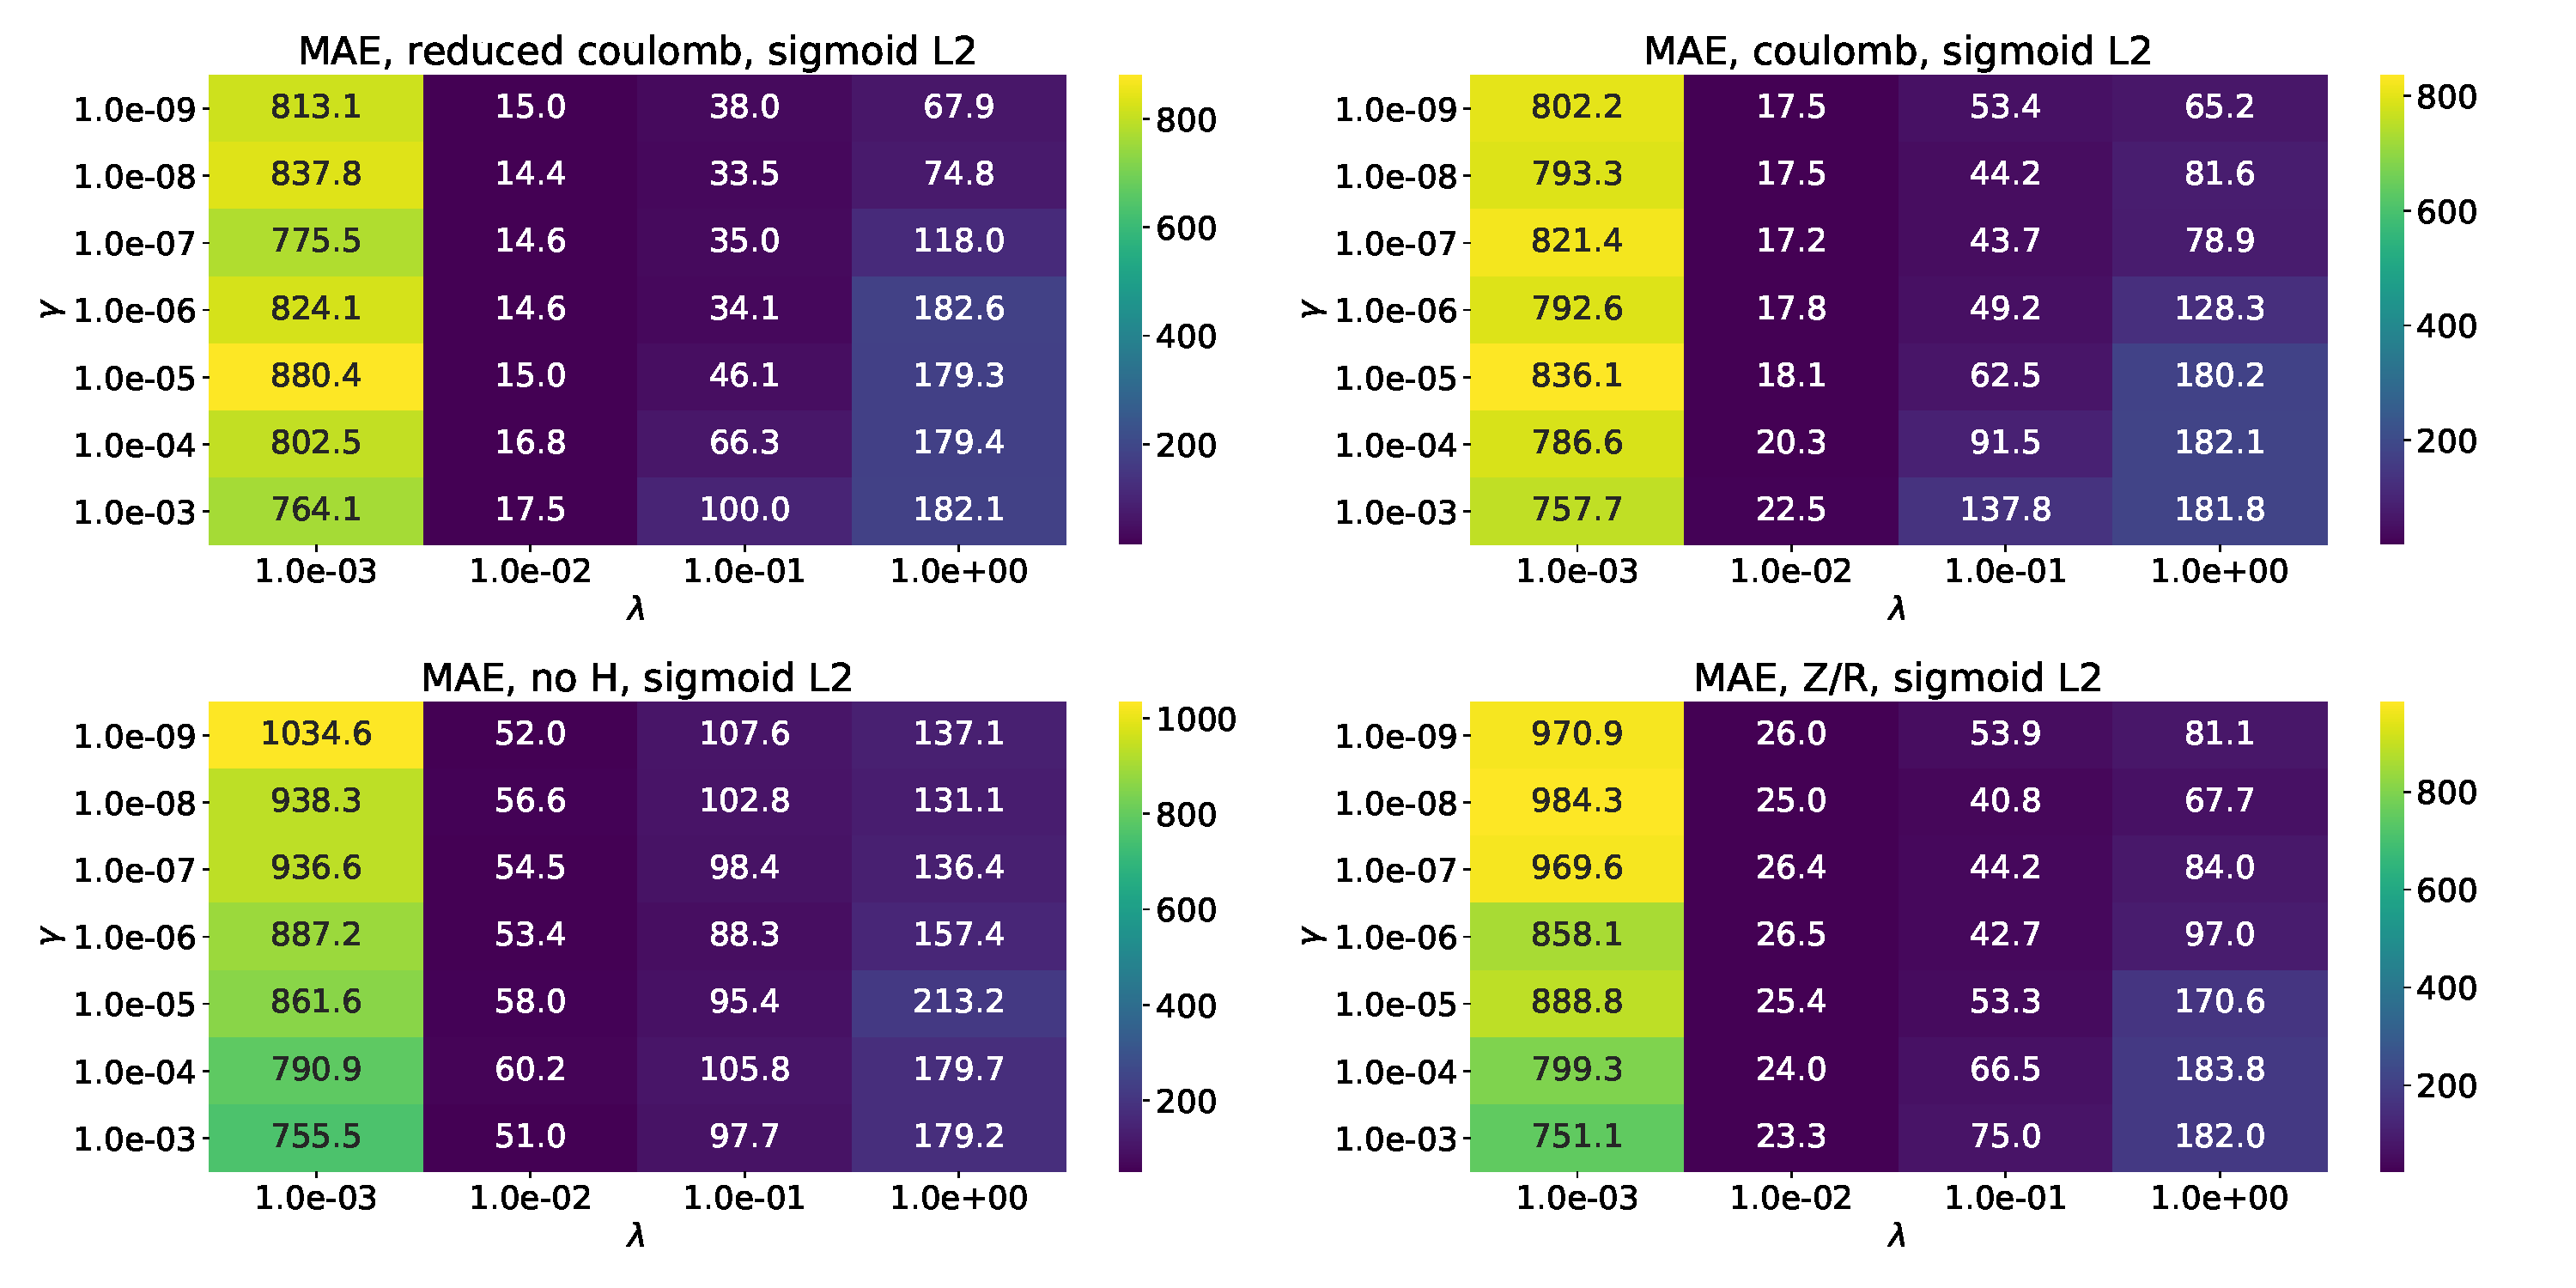
\includegraphics[width=1\textwidth]{nn_100_sigmoid L2.pdf}
\caption[NN, sigmoid L2, 100 epochs]{Test MAE using the 4 different representations as function of the learning rate $\gamma$ and the regularisation rate $\lambda$ using L2 regularization and the sigmoid activation function. The Neural Network consisted of two 100-neuron layers and was trained for 100 epochs.} \label{fig:sigmoid_l2_100}
\end{figure}
\begin{figure}[H]
\centering
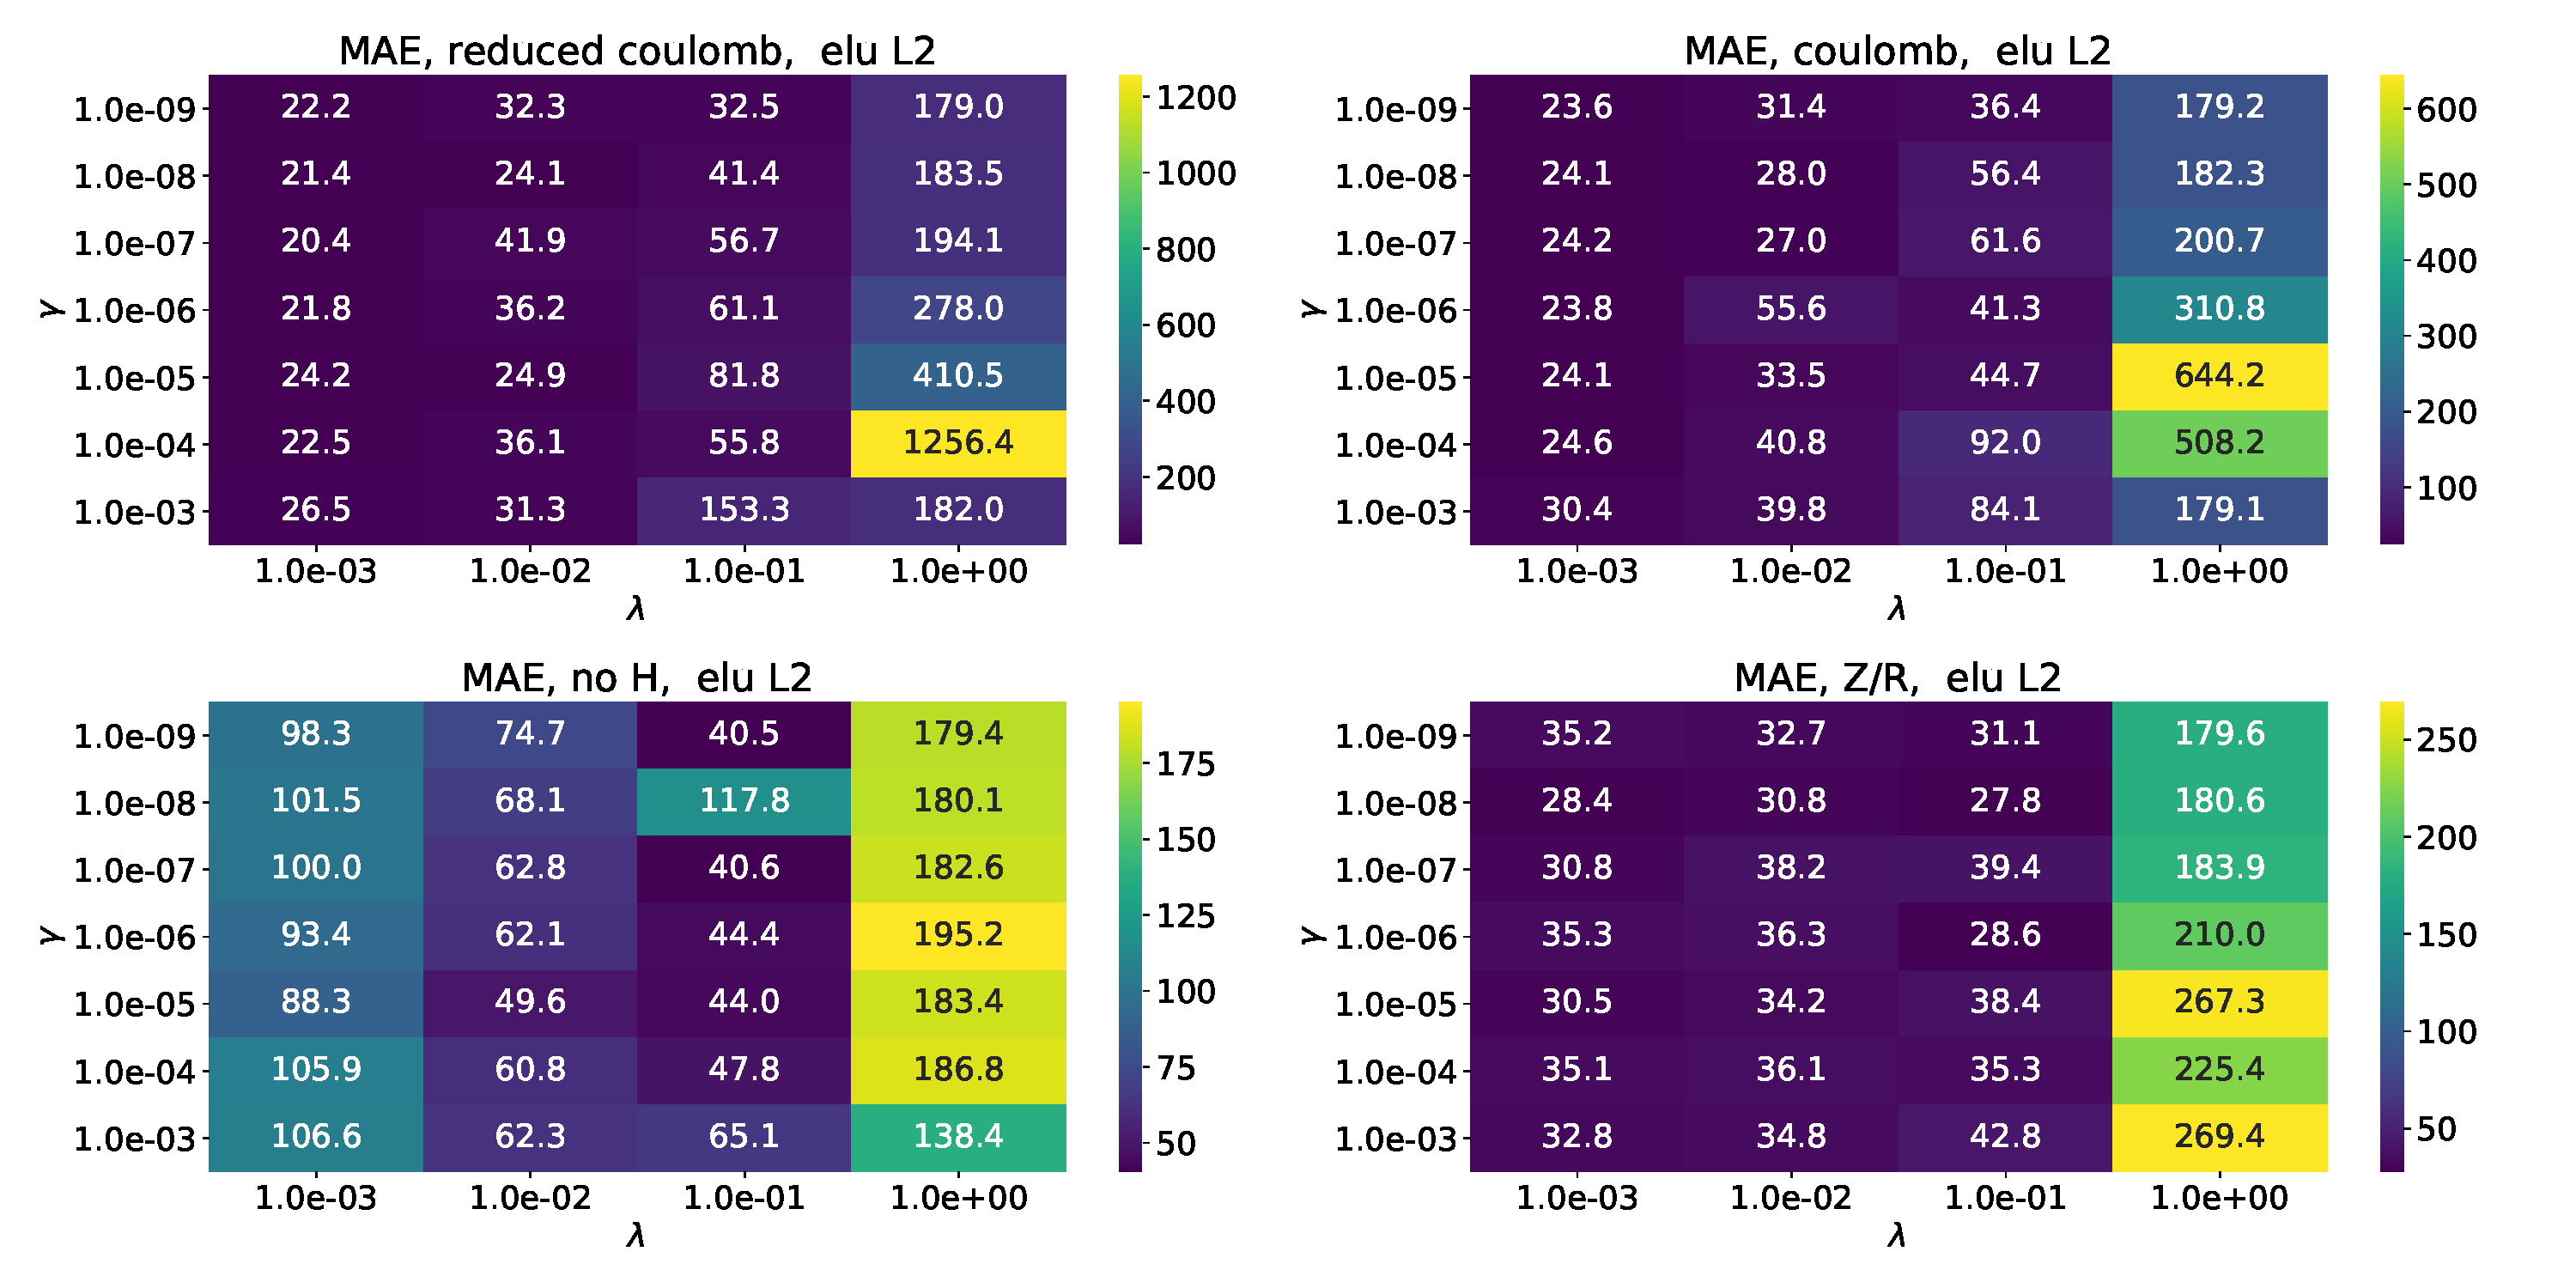
\includegraphics[width=1\textwidth]{nn_100_ elu L2.pdf}
\caption[NN, elu L2, 100 epochs]{Test MAE using the 4 different representations as function of the learning rate $\gamma$ and the regularisation rate $\lambda$ using L2 regularization and the elu activation function. The Neural Network consisted of two 100-neuron layers and was trained for 100 epochs.} \label{fig:elu_l2_100}
\end{figure}
\begin{figure}[H]
\centering
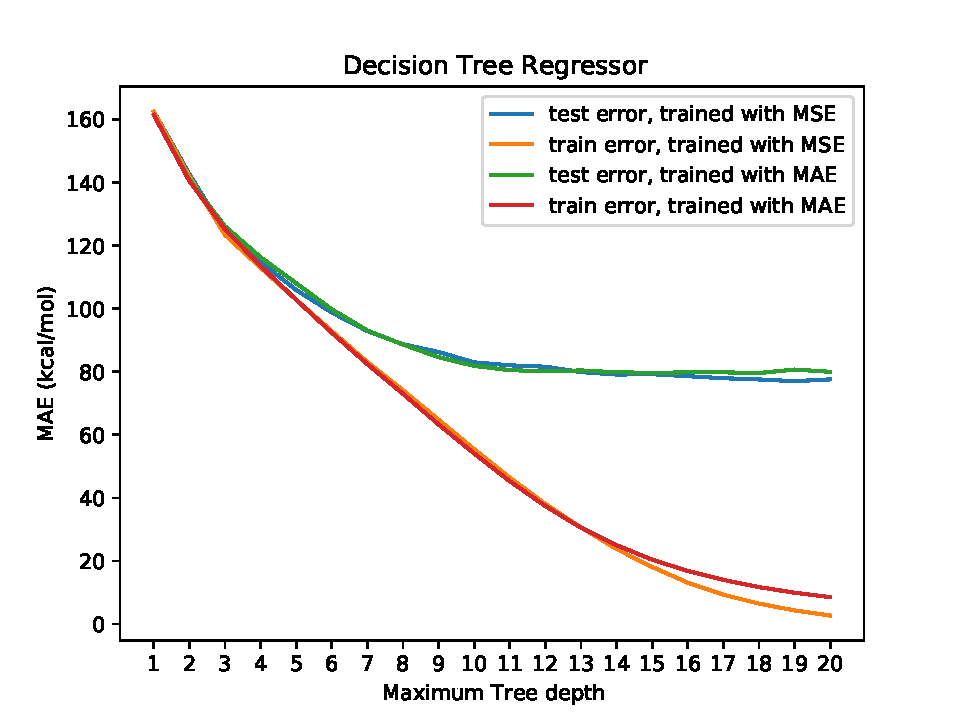
\includegraphics[width=0.8\textwidth]{decision_treenoH.pdf}
\caption[Decision Tree, no H]{Test and Train MAE using 5-fold Cross-Validation for a Decision Tree, using the CART algorithm to minimize either MSE or MAE, as function of the maximum tree depth for the Hydrogen-free approach.} \label{fig:decisiontreenoH}
\end{figure}

\begin{figure}[H]
\centering
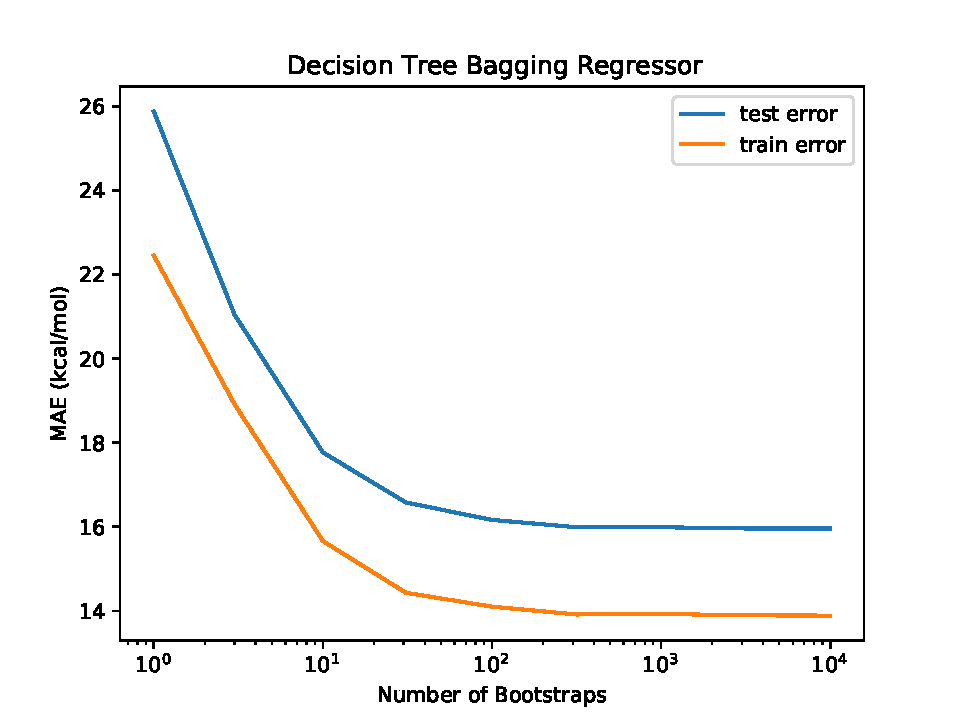
\includegraphics[width=0.8\textwidth]{bagging_2.pdf}
\caption[Bad Bagging]{Test and Train MAE using 5-fold Cross-Validation for Bagging as function of the number of Trees grown with Decision Trees as weak Learners, where we used trees of max depth 7, using only 1000 samples. The CART algorithm was used to minimize the MSE for each tree.} \label{fig:bagging_2}
\end{figure}
\begin{figure}[H]
\centering
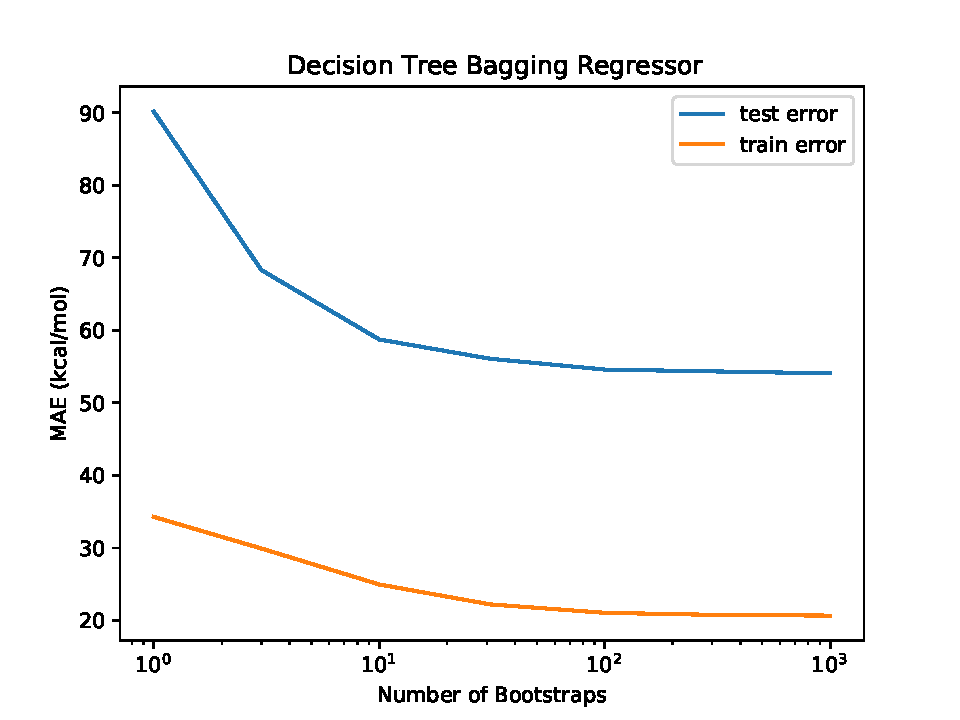
\includegraphics[width=0.8\textwidth]{bagging_2noH.pdf}
\caption[Bagging, no H]{Test and Train MAE using 5-fold Cross-Validation for Bagging as function of the number of Trees grown with Decision Trees as weak Learners for the Hydrogen-free approach, where we used trees of max depth 20. The CART algorithm was used to minimize the MSE for each tree.} \label{fig:baggingnoH}
\end{figure}
\begin{figure}[H]
\centering
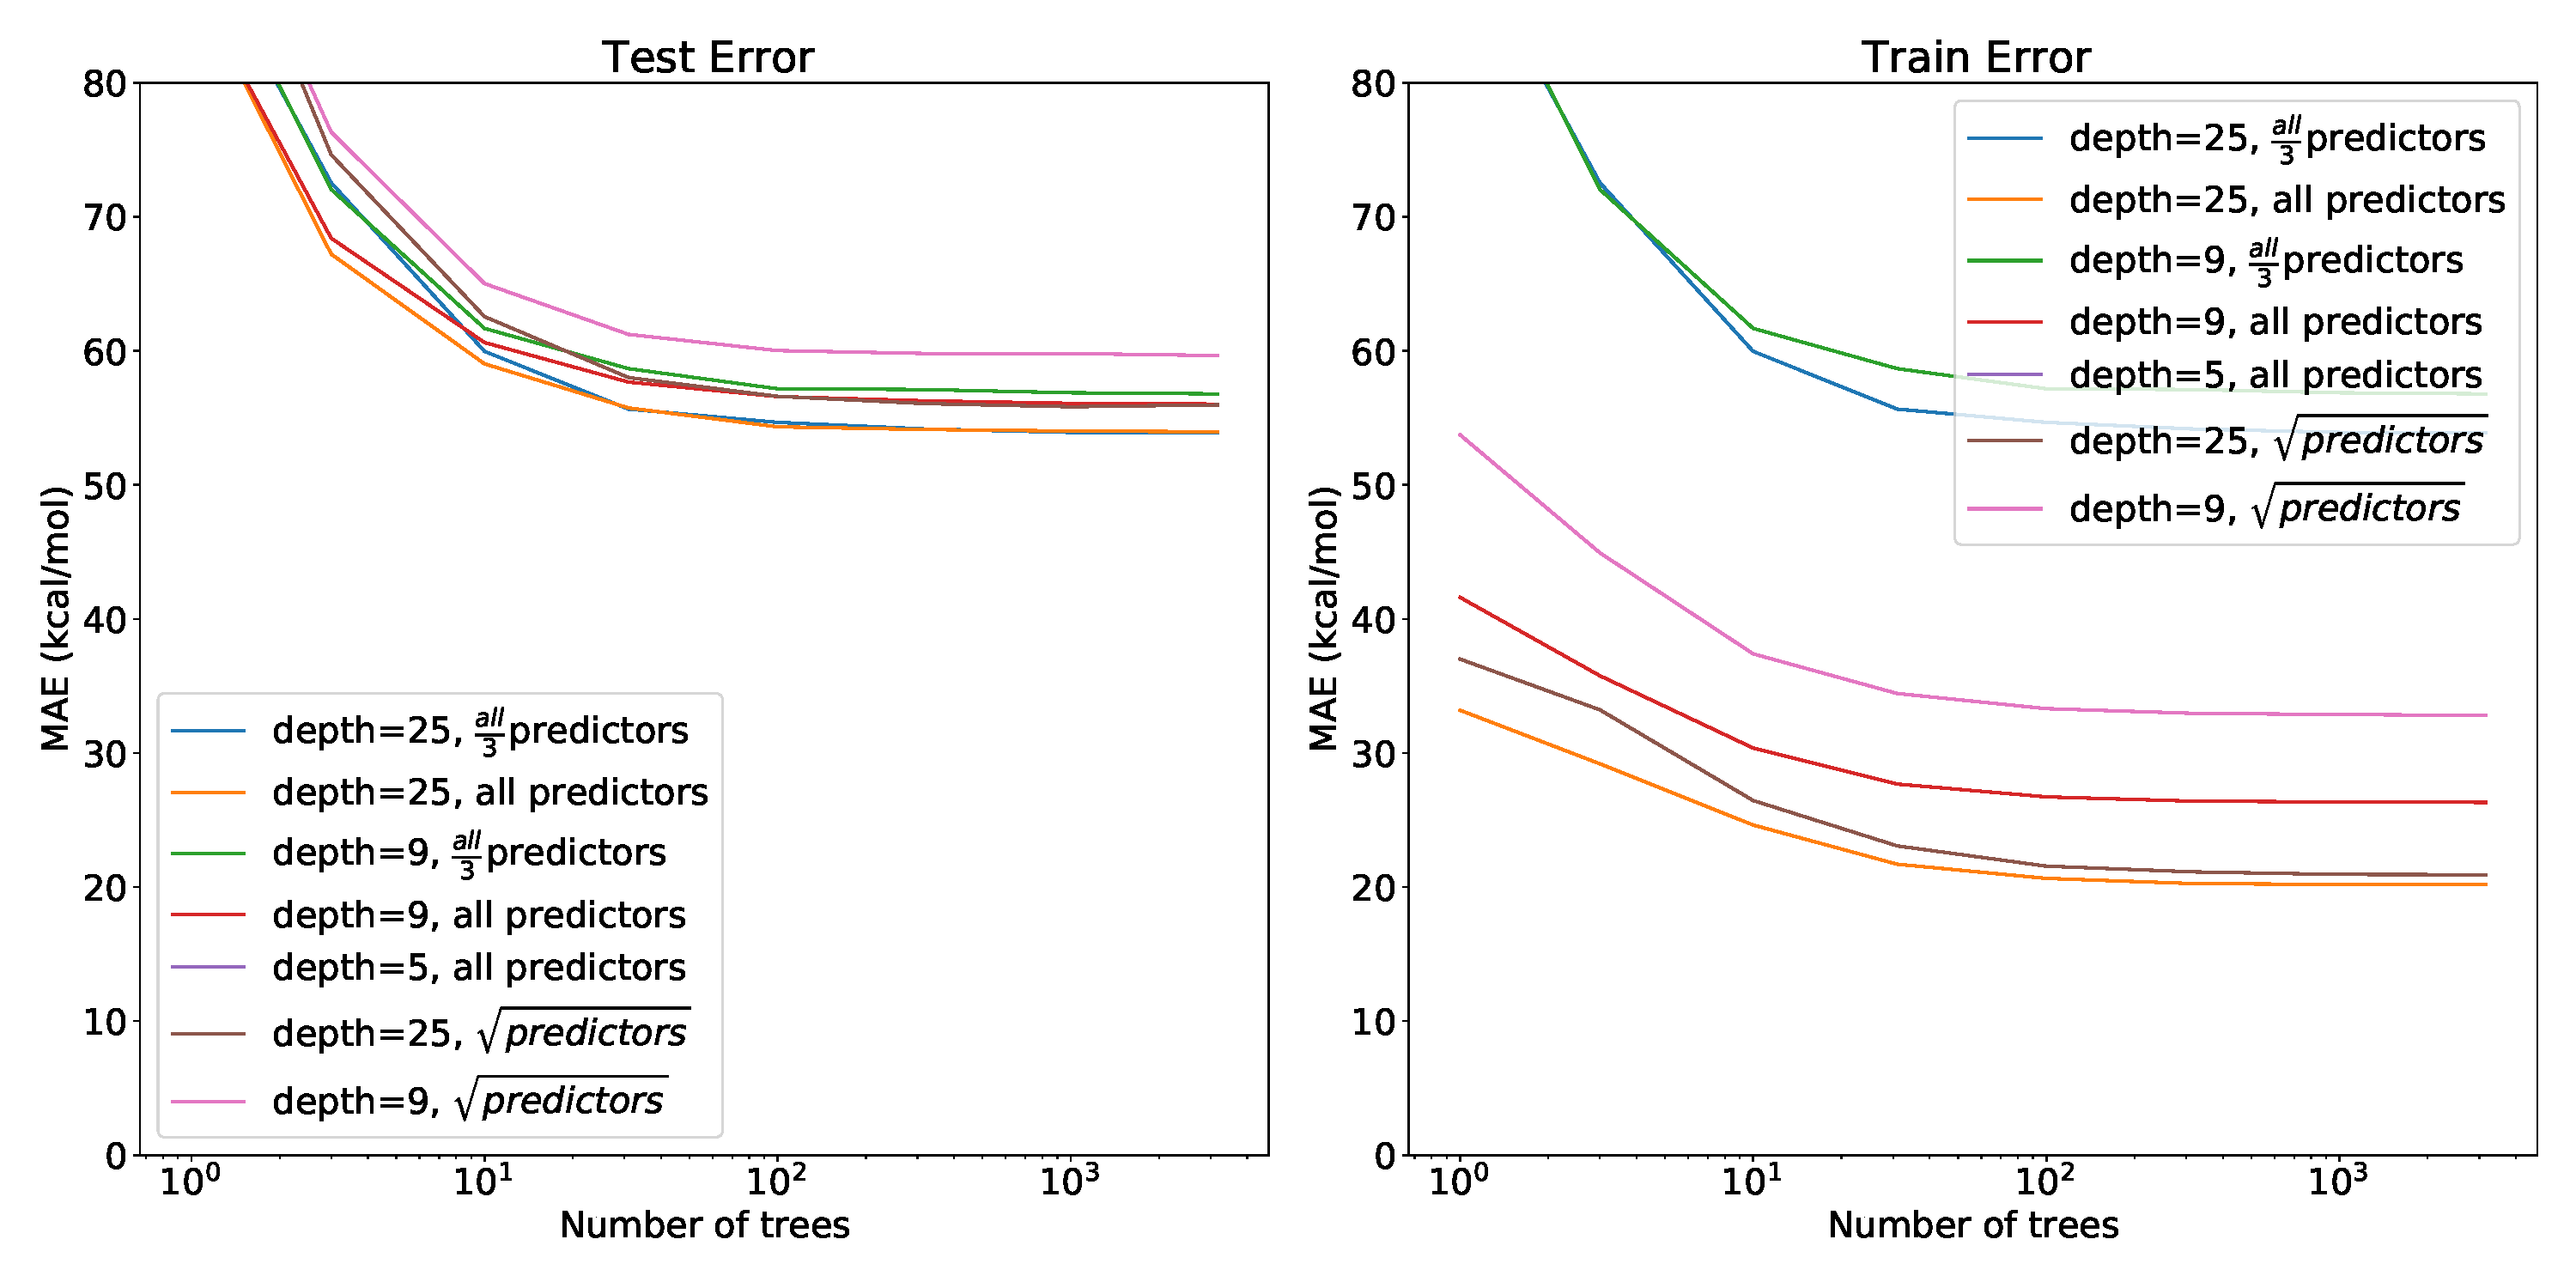
\includegraphics[width=0.8\textwidth]{forestnoH.pdf}
\caption[Random Forests, no H]{Test and Train MAE using 5-fold Cross-Validation for Random Forest as function of the number of Trees grown with Decision Trees as weak Learners for the Hydrogen-free approach, where we used trees of different max depths with different numbers of predictors being used. The CART algorithm was used to minimize the MSE for each tree.} \label{fig:randomforestnoH}
\end{figure}

\begin{figure}[H]
\centering
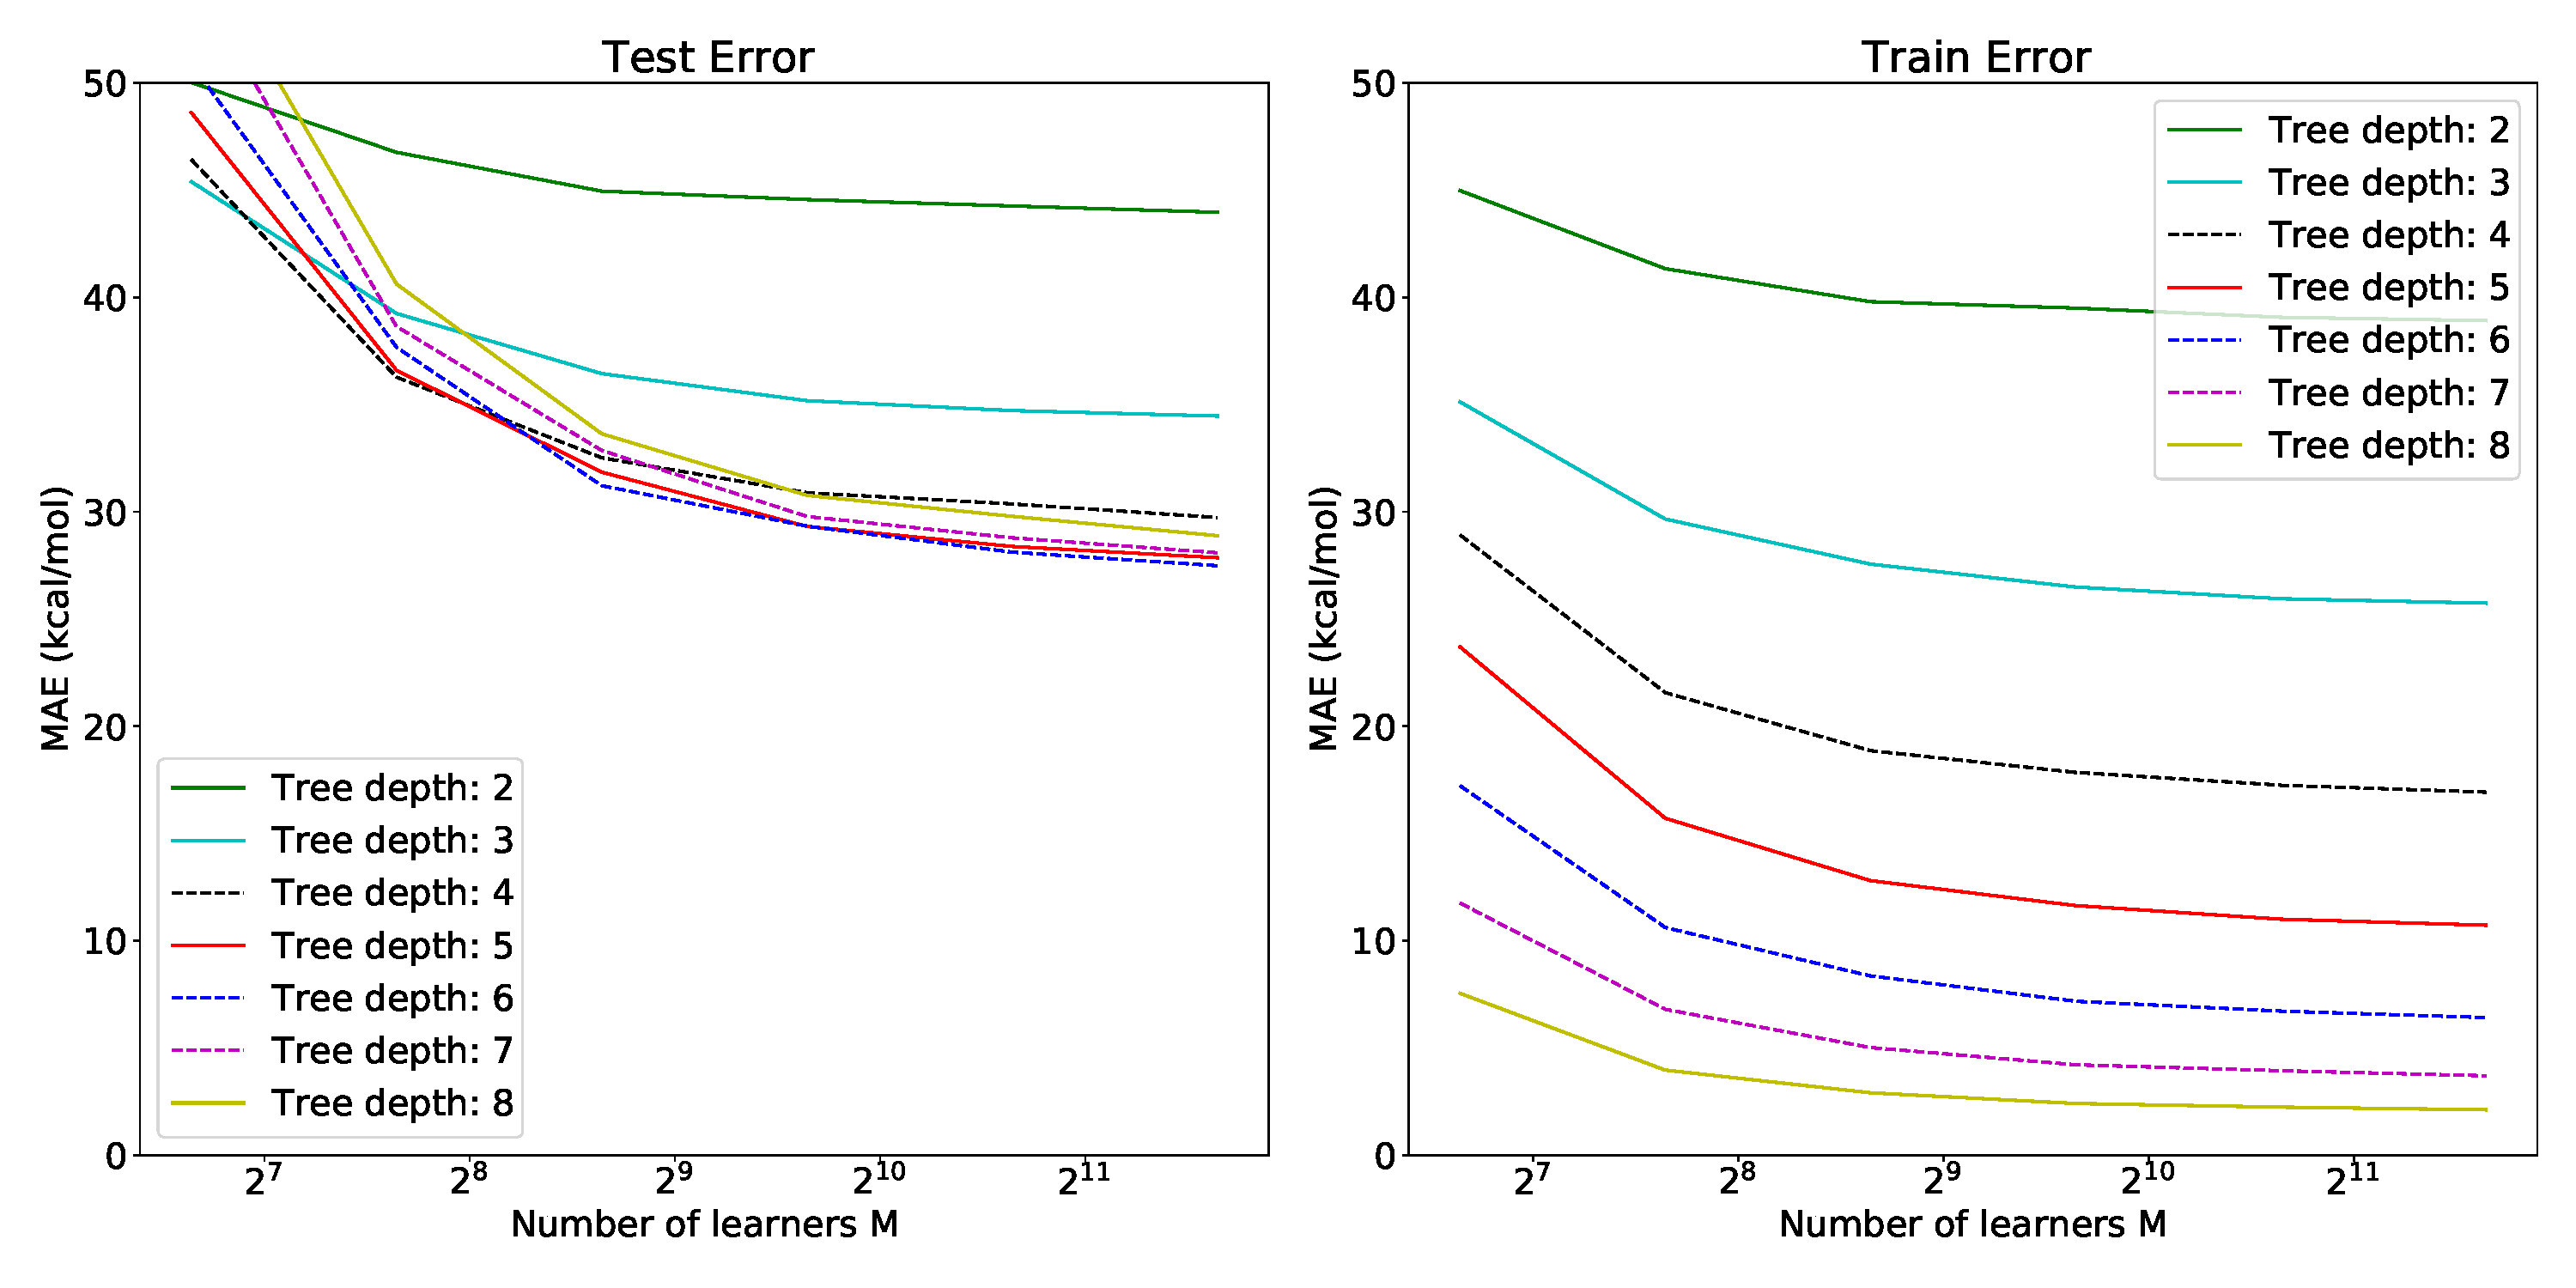
\includegraphics[width=1\textwidth]{boosting1noH.pdf}
\caption[Boosting $M\eta=50$, no H]{Test and Train MAE using 5-fold Cross-Validation for Boosting as function of the number of Trees grown with Decision Trees as weak Learners on the Hydrogen-free Coulomb matrix, where we used trees with variable maximum depth (see label). We used a L1 regularisation of $\lambda_{L1}=10$, sampled 50\% of samples and 30\% of features, and adapted the learning rate $\eta=50/M$.} \label{fig:boosting3}.
\end{figure}

\bibliographystyle{plain}
\bibliography{references}
\end{document}
